Ein wesentlicher Teil dieser Arbeit besteht in der softwareseitigen Realisierung
der Laserstabilisierung und Experimentsteuerung. In diesem Kapitel sollen daher
alle Softwarekomponenten genauer betrachtet werden. In Abschnitt
\ref{sec:datenerfassung_der_laser} wird beschrieben, wie die Informationen
der Laserfrequenzen aus der Counterkarte ausgelesen, im
Mikrocontroller \textit{Arduino} aufbereitet und anschließend am PC ausgewertet
werden. In Abschn. \ref{sec:stabilisierung_frequenzverstimmungs-strategie} wird die Regelung
der Laserfrequenz und die damit verbundene Strategie der Frequenzverstimmung
erklärt. Abschnitt \ref{sec:linearisierung_iscan} beschäftigt sich mit der
Linearisierung der \textit{iScans} und dem Neuschreiben der LUT. Die
Benutzerschnittstelle zur Experimentsteuerung soll in Abschn.
\ref{sec:experimentsteuerung} behandelt werden. In Abschn. \ref{sec:sonstiges}
werden weitere Funktionen kurz angerissen. Da die Software am PC in
\textit{Labview} entwickelt wurde und somit der Code nur sehr unübersichtlich
dargestellt werden kann, wird die Beschreibung ausschließlich über
Ablaufdiagramme und Bildschirmfotos der Benutzeroberfläche geschehen. Der
Quellcode des \textit{Labview}-Programms kann am Kontrollrechner selbst eingesehen
werden. Programme in \textit{Labview} werden im Folgenden \textit{Virtuelles
Instrument} (VI) bzw. SubVI (Unterprogramm) genannt. SubVIs sind standardmäßig
nichts anderes als ausgelagerte Codestücke und sind für die Zeit, in der sie
verwendet werden, gesperrt. Dies unterscheidet \textit{Labview} wesentlich von
anderen Programmiersprachen. Es gibt jedoch die Möglichkeit ein SubVI als
\textit{reentrant}\footnote{http://zone.ni.com/devzone/cda/tut/p/id/6411}
(eintrittsinvariant oder wiedereintrittsfähig) zu deklarieren. Wird das SubVI
dann mehrfach in einem übergeordneten VI verwendet, werden dieser SubVI
entsprechend viele Kopien des Speicherbereichs zur Verfügung gestellt. Dies ist vergleichbar mit dem Instanziieren von Klassen
in anderen Programmiersprachen und macht ein unabhängiges Ausführen möglich.
Dies führt gerade bei PC-Systemen mit viel Arbeitsspeicher und einem Prozessor, der
Prozesse bzw. Threads parallel ausführen kann, zu enormen
Performancesteigerungen.
Aus diesen Gründen wurde darauf geachtet, dass mehrfach verwendete SubVIs
inbesondere bei der Laserkontrolle reentrant sind.

\section{Datenerfassung der Laser}\label{sec:datenerfassung_der_laser}
Die Informationen über die Laser durchlaufen mehrere Stufen der Signal- und
Datenverarbeitung, bis eine quantitative Aussage über das Frequenzverhalten
gemacht werden und eine Regelroutine anlaufen kann. Der erste Teil der
Datenaufbereitung verläuft rein elektronisch, bis die Counterwerte binär in
den Counterregistern abrufbereit vorliegen, wie bereits in Abschn.
\ref{sec:elektronik_laserkontrolle} ausführlich erklärt wurde. An dieser Stelle
setzt nun die softwareseitige Weiterverarbeitung an. Im Folgenden wird sich
wieder exemplarisch nur auf einen Diodenlaser und den Referenzlaser bezogen.
Für alle anderen Laser gilt der identische Ablauf.

\subsection{Datenaufbereitung}\label{subsec:datenaufbereitung}
Zunächst werden die Counterwerte mithilfe des Mikrocontrollers \textit{Arduino}
ausgelesen und verarbeitet. Das komplette Ablaufdiagramm der Software des
\textit{Arduinos} ist in Abb. \ref{fig:ablaufdiagramm_arduino_laser} in auf die
wesentlichen Teile gekürzter Form zu sehen. Der komplette Quellcode hierfür
wurde in der Programmiersprache C geschrieben und ist im Anhang
\ref{anh:sec:quelltext_arduino_laserinformationsverarbeitung} zu finden.
\begin{figure}[hp]
 	\centering
 	\fbox{\parbox{\dimexpr \linewidth - 2\fboxrule - 2\fboxsep}{
 	\centering
	    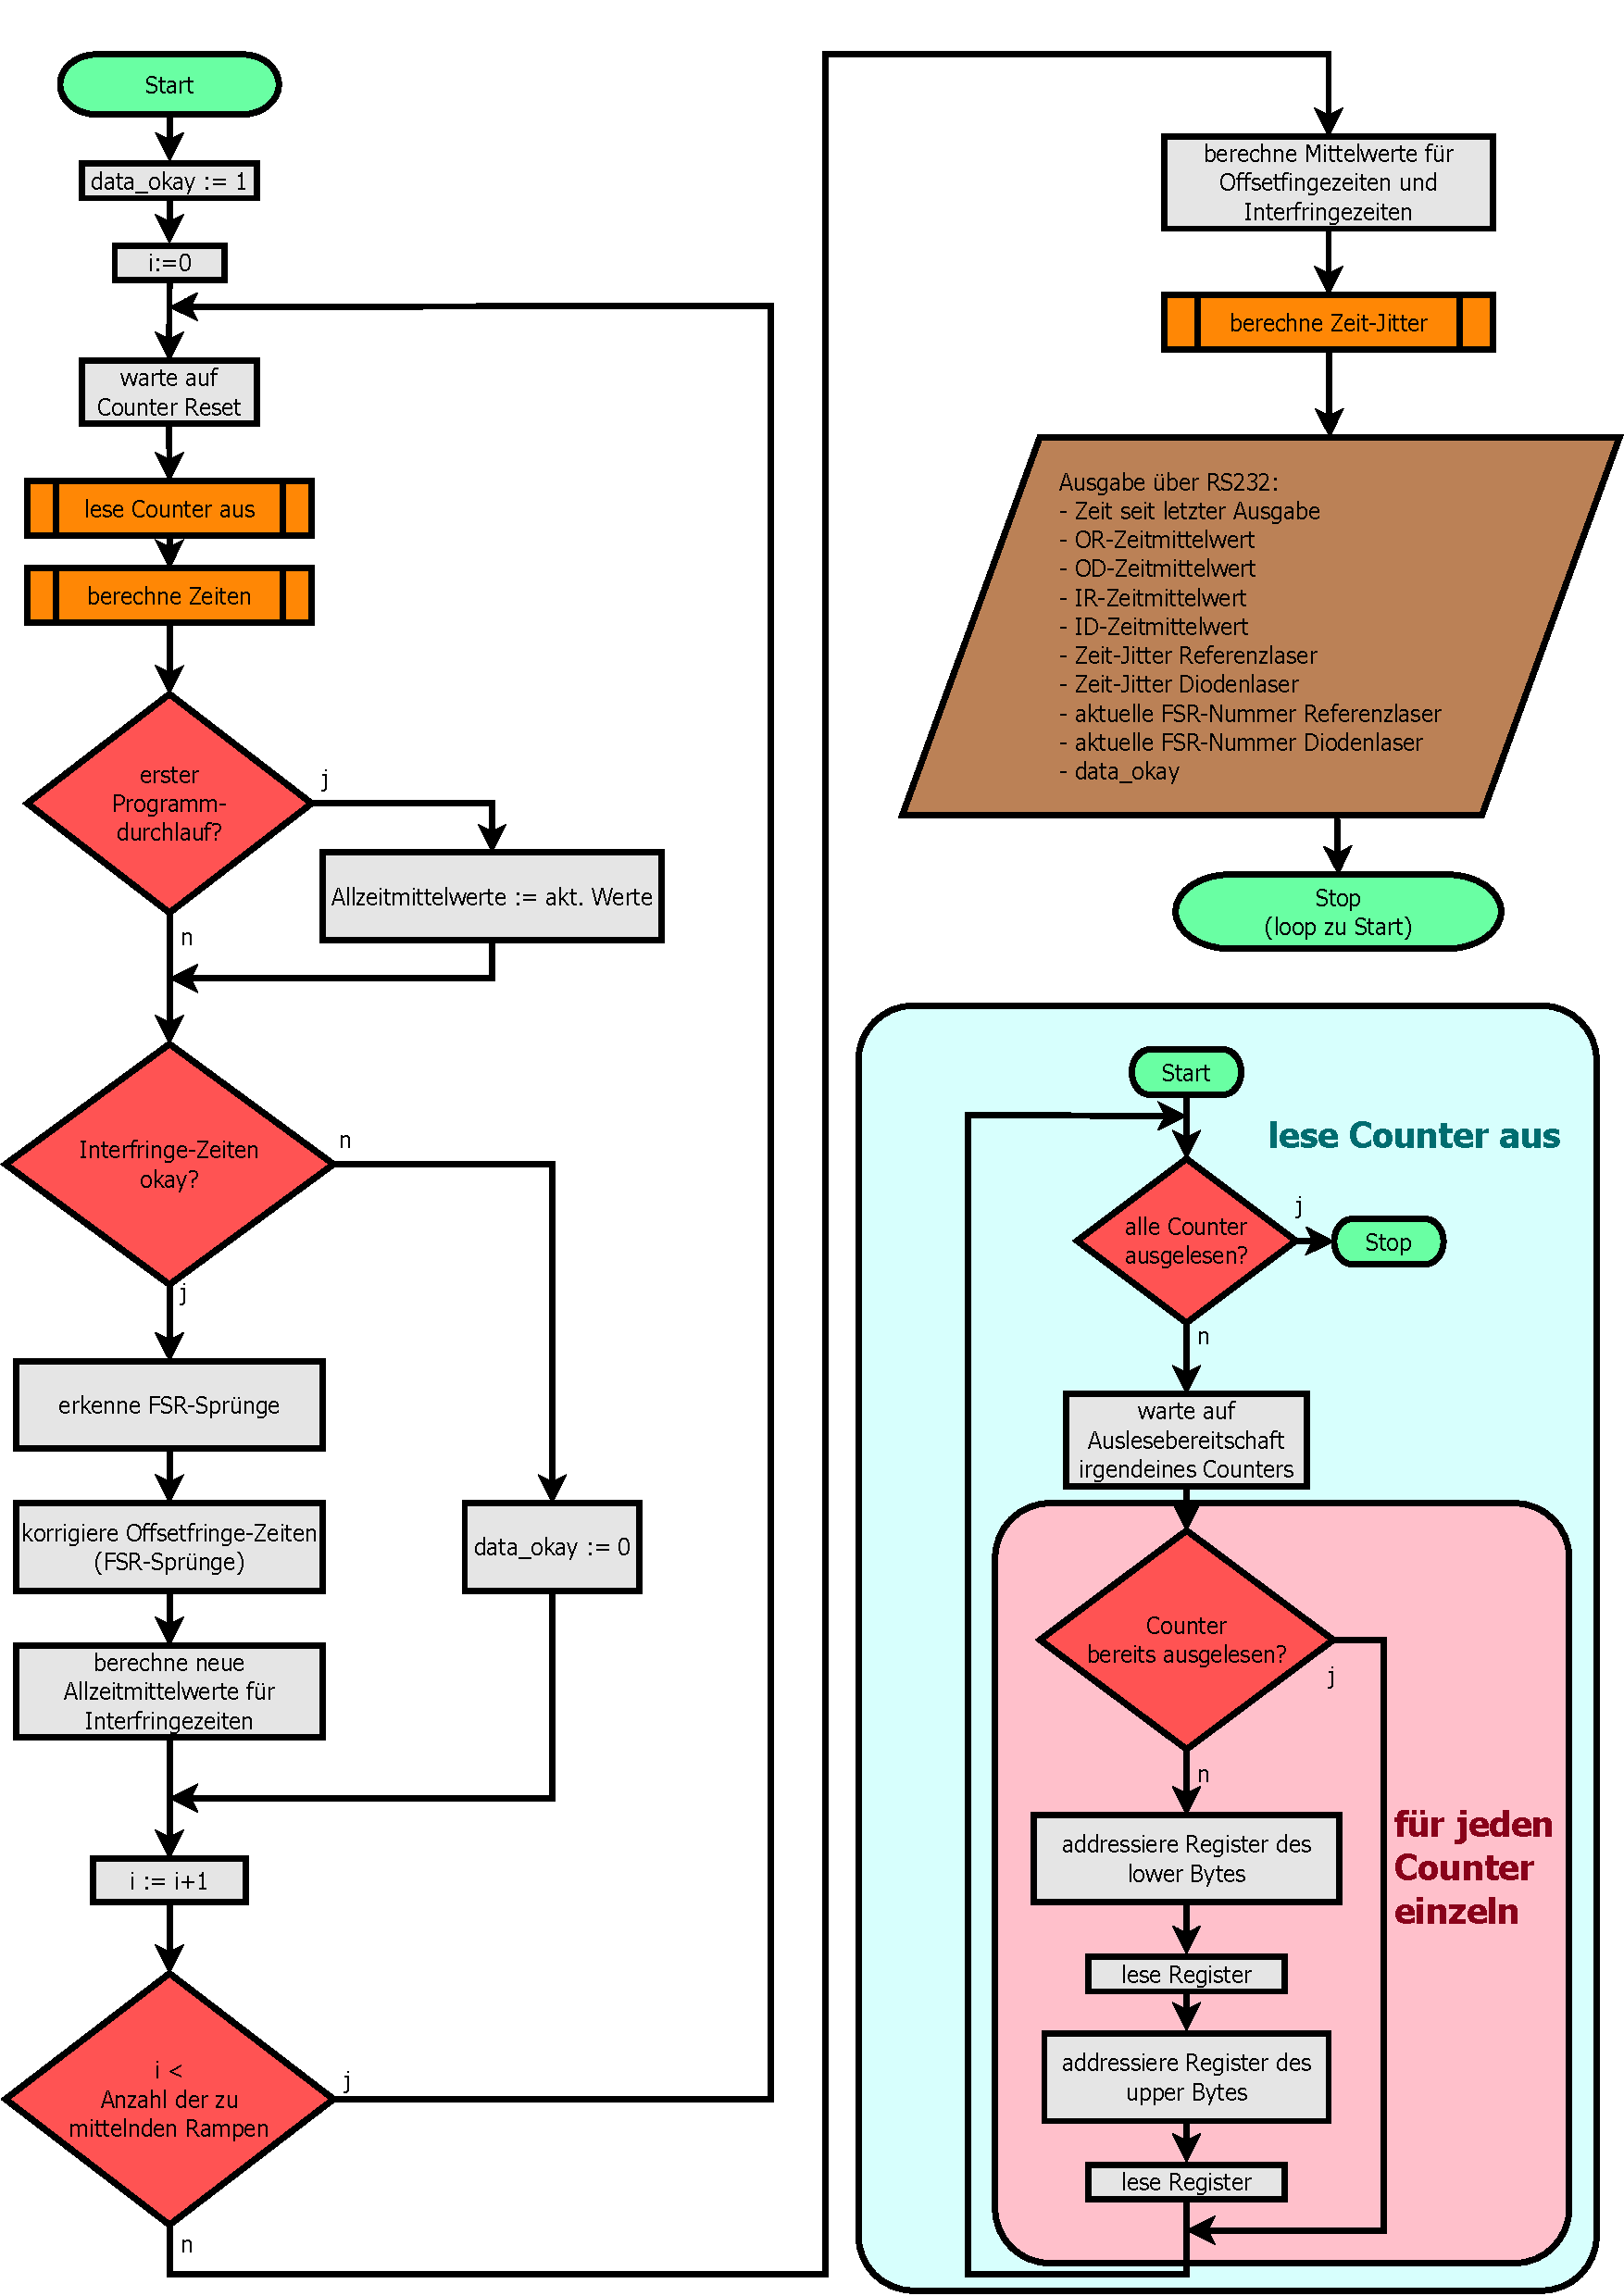
\includegraphics[width=\textwidth-0.5cm]{gfx/ablaufdiagramm_arduino_laser}
	    }}
	\caption[Laserdatenaufbereitung -
	Ablaufdiagramm]{Ablaufdiagramm der Laserdatenaufbereitung mit dem
	\textit{Arduino}. (j=ja, n=nein)}
	\label{fig:ablaufdiagramm_arduino_laser}
\end{figure}
Der \textit{Arduino} verfügt über 54 digitale Ein- und Ausgänge, welche der
Kommunikation mit der Counterkarte dienen. HIGH ($5\,$V) bzw. LOW ($0\,$V) wird
als 1 bzw. 0 oder TRUE bzw. FALSE interpretiert. Das Programm besteht aus
einem
\textit{Setup}, in dem initialisierende Routinen wie beispielsweise die
Pinbelegung abgearbeitet werden, und einer \textit{Endlosschleife} (\textit{Start}$\rightarrow$\textit{Programm}$\rightarrow$\textit{Stop}$\rightarrow$\textit{Start}$\rightarrow$\ldots),
über die die stetige Überwachung der Laser abgewickelt wird. Die Aufgaben des
Programms sind
\begin{itemize}
	\item Counter auslesen
	\item reale Zeiten berechnen
	\item unplausible Zeiten ignorieren
	\item FSR-Sprünge erkennen und Zeiten korrigieren
	\item Mittelwerte der Zeiten bilden.
	\item Laser-Jitter berechnen.
\end{itemize}
All dies muss innerhalb eines Rampenzyklus (also innerhalb von maximal
$17\,$ms) geschehen, damit keine Information verloren geht. Im schlimmsten Fall
bleiben dem Mikrocontroller für die Berechnungen nach dem Auslesen der Counter
nur ca. $2\,$ms (fallende Rampe). Aus diesem Grund wurde das Programm möglichst
effizienz gestaltet.\par
Es wird stets eine bestimmte Anzahl von
Rampenzyklen zusammengefasst und Zeitmittelwerte für die Offset- und Interfringezeiten beider Laser ($t_{OR,i}$, $t_{OD,i}$, $t_{IR,i}$ und $t_{ID,i}$) berechnet. Weiterhin wird aus der
Standardabweichung der Offsetfringezeiten der Jitter
\begin{equation}\label{eq:jitter_zeit}
	\Delta
	t_O=\sqrt{\frac{1}{n-1}\cdot\sum\limits_{i=1}^{n}\left(t_{O,i}-\overline{t}_O\right)^2}
\end{equation}
des jeweiligen Lasers über die Anzahl der zu mittelnden Rampenzyklen
ermittelt.\par
Eine Iteration beginnt - wenn nötig - mit dem Warten bis alle
Counter zurückgesetzt wurden, indem geprüft wird, ob alle Status-Bits LOW sind,
was während der fallenden Rampe geschieht.
Anschließend werden die Counter ausgelesen. Dabei wird in einer Schleife zu
Beginn geprüft, ob bereits alle Counter ausgelesen worden sind. Wenn dies nicht
der Fall ist, wird über die Status-Bits auf die Bereitschaft irgendeines
Counters gewartet und im Falle der Bereitschaft geprüft, ob der Counter schon
ausgelesen worden ist. Wurden die Werte noch nicht ausgelesen, werden upper und
lower Byte nacheinander adressiert und ausgelesen.\par
Aus den erhaltenen 16-Bit-Werten werden nun über die fest einprogrammierte
Taktrate die wirklichen Zeiten berechnet. Während der gesamten Laufzeit des
Programms werden nach jeder Iteration
Langzeitmittelwerte\footnote{Die Langzeitmittelwerte sind Mittelwerte der
Interfringezeiten für alle Werte von Beginn der Programmlaufzeit. Sie werden
mit den Zeiten im ersten Durchlauf initiiert und danach permanent mit gültigen
Werten aktualisiert.} für die Interfringezeiten erneuert.
Zu Beginn des Programms werden diese mit den ersten Zeiten initialisiert. Mithilfe der Langzeitmittelwerte wird geprüft, ob die
aktuellen Interfringezeiten valide sind. Es kann insbesondere bei schnellen
Frequenzverstimmungen vorkommen, dass während einer Rampe der Interfringe aus
dem aktuellen FSR hinausläuft, noch bevor der Counter gestoppt wurde und
somit eine falsche Zeit gemessen wird. Um diese Fälle und andere Fehlmessungen
auszusondern, wird geprüft, ob die gemessene Interfringezeit stark vom
Langzeitmittelwert abweicht. Bei offensichtlich falscher Messung wird die
momentane Iteration abgebrochen und für die spätere Ausgabe eine
Validitätsvariable auf 0 gesetzt, damit bei der Weiterverarbeitung am PC
entschieden werden kann, ob die Daten genutzt werden möchten oder nicht.\par
Sind die Zeiten valide, kann herausgefunden werden, ob die Laserfrequenz des
Diodenlasers in einen benachbarten FSR des FPIs gelaufen ist. Dabei wird
überprüft, ob sich die Zeit des Offsetfringes relativ gemessen zur
Offsetfringezeit des Referenzlasers gegenüber der Zeit der vorherigen Rampe um mehr als die Hälfte der Interfringezeit verändert hat. Folgendes kann auftreten:
\begin{subequations}\label{eq:FSR-sprung}
	\begin{equation}\label{eq:FSR-sprung_links}
		(t_{OD,akt.}-t_{OR,akt.})-(t_{OD,alt}-t_{OR,alt})>\nicefrac{1}{2}\cdot
t_{ID,akt}
	\end{equation}
	\begin{equation}\label{eq:FSR-sprung_rechts}
		(t_{OD,akt.}-t_{OR,akt.})-(t_{OD,alt}-t_{OR,alt})<-\nicefrac{1}{2}\cdot
t_{ID,akt}\,.
	\end{equation}
\end{subequations}
Gilt \eqref{eq:FSR-sprung_links}, so wird vermutet, dass der Laser in den links
benachbarten FSR gedriftet ist. Im Falle von \eqref{eq:FSR-sprung_rechts} ist
der Laser vermutlich in den rechts benachbarten FSR gedriftet. In
beiden Fällen wird eine FSR-Nummer-Variable erniedrigt bzw. erhöht, um später am
PC die FSR-Sprünge zählen zu können. Die Detektion kann natürlich wie schon
erwähnt nur funktionieren, wenn die Frequenz deutlich langsamer als
$\nicefrac{\text{FSR}}{2}$ pro Rampenzyklus verstimmt wird. Damit auch bei
FSR-Sprüngen die Zeiten zur Mittelung beitragen können, werden diese
anschließend durch Subtrahieren bzw. Addieren der Interfringezeit korrigiert.\par
Für den Referenzlaser ist ein FSR-Sprung aufgrund seiner absoluten Stabilität
bis auf wenige MHz praktisch unmöglich, sofern der Offset der Rampe so
eingestellt ist, dass der erste Fringe ca.
$\nicefrac{\text{FSR}}{2}$ nach Start der Rampe auftaucht. Somit bleibt die
Laserfrequenz mit aller Sicherheit immer in demselben FSR des FPIs. Es
kommt jedoch vor, dass die Rampe oder das FPI einer Drift unterliegen
und der Referenzlaser scheinbar in einen benachbarten FSR driftet.
Analog wie beim Diodenlaser wird auch hier der scheinbare FSR-Sprung
detektiert. In diesem Fall wird aber lediglich die Offsetfringezeit wie beim
Diodenlaser korrigiert. Die Zählvariable für den scheinbaren FSR-Sprung
wird nur noch zu Debugzwecken aufbewahrt. Logischerweise können
gleichzeitige FSR-Sprünge beider Laser so nicht erkannt werden. In diesem
sehr unwahrscheinlichen Fall käme es zu Fehlberechnungen der Relativfrequenz.
Um dennoch sicher zu sein, sollte deshalb regelmäßig auf die Lage des ersten
He:Ne-Fringes geachtet und ggf. das Offset der Rampe nachkorrigiert werden.\par
Wurden genügend Rampen durchlaufen, können die aktuellen Mittelwerte aller
Zeiten und die Standardabweichung der Offsetfringezeiten berechnet und mit allen
anderen nötigen Werten über eine RS232-Schnittstelle an den PC gesandt werden
(brauner Kasten in Abb.
\ref{fig:ablaufdiagramm_arduino_laser}). Der versandte String beginnt
mit \lstinline|"*begin*"| und endet mit \lstinline|"*end*"|, damit später
sichergestellt werden kann, wo die Daten anfangen und aufhören. Die Werte sind
untereinander durch Leerzeichen getrennt.

\subsection{Datenbereitstellung am PC}\label{subsec:datenbereitstellung}
Die Daten eines jeden Lasers kommen, wie oben erwähnt, als String in
Zeitabständen eines Vielfachen der Rampendauer am PC an. Damit es zu keinem Pufferstau an
der seriellen Schnittstelle des PCs kommt, werden die aktuellen Strings direkt
nach Abschneiden von \lstinline|"*begin*"| und \lstinline|"*end*"| durch das
SubVI \lstinline|arduino_laser_read.vi| in globale Variablen geschrieben.
Parallel wird jeweils eine boolsche Variable gesetzt, die angibt, dass die Laserinformationen aktuell sind. Wird ein String aus einer der
globalen Variablen gelesen, wird die boolsche Variable zurückgesetzt und die
Laserinformationen werden als nicht mehr aktuell gewertet. Aktualität fordernde
Lesezugriffe auf die Daten warten, bis die Variable wieder gesetzt wurde. Die
Piorität liegt hier auf der Aktualität der Daten und nicht darauf, möglichst
jedes Datenpaket zu verarbeiten. Die aktuellen Zeiten können nun separat über
das SubVI \lstinline|get_laser_times.vi| nach Angabe der Lasernummer abgeholt werden. Das SubVI \lstinline|delta_time2delta_frequency.vi| berechnet nach Gl. \eqref{eq:FPI_frequenzdrift_03} aus den Zeiten die Relativfrequenzen. Das SubVI \lstinline|laser-control.vi|, das in Abschn.
\ref{sec:stabilisierung_frequenzverstimmungs-strategie} näher betrachtet wird,
hat neben der Regelung und Frequenzverstimmung auf die Sollfrequenz auch die Aufgabe, Monitoringdaten an die Benutzeroberfläche der Laserkontrolle (Abb.
\ref{fig:benutzeroberflaeche_laserkontrolle}) weiterzugeben. Zu den
Monitoringdaten gehören Jitter des Lasers, Ist-Relativfrequenz und Abweichung
zur Soll-Relativfrequenz, wobei die detektierten FSR-Sprünge mit einbezogen
werden müssen. Die Referenzfrequenz ist beim Start des Programms oder beim
Drücken des Buttons \lstinline|assign| die derzeit aktuelle Laserfrequenz.
\begin{figure}[h]
 	\centering
 	\fbox{\parbox{\dimexpr \linewidth - 2\fboxrule - 2\fboxsep}{
 	\centering
	    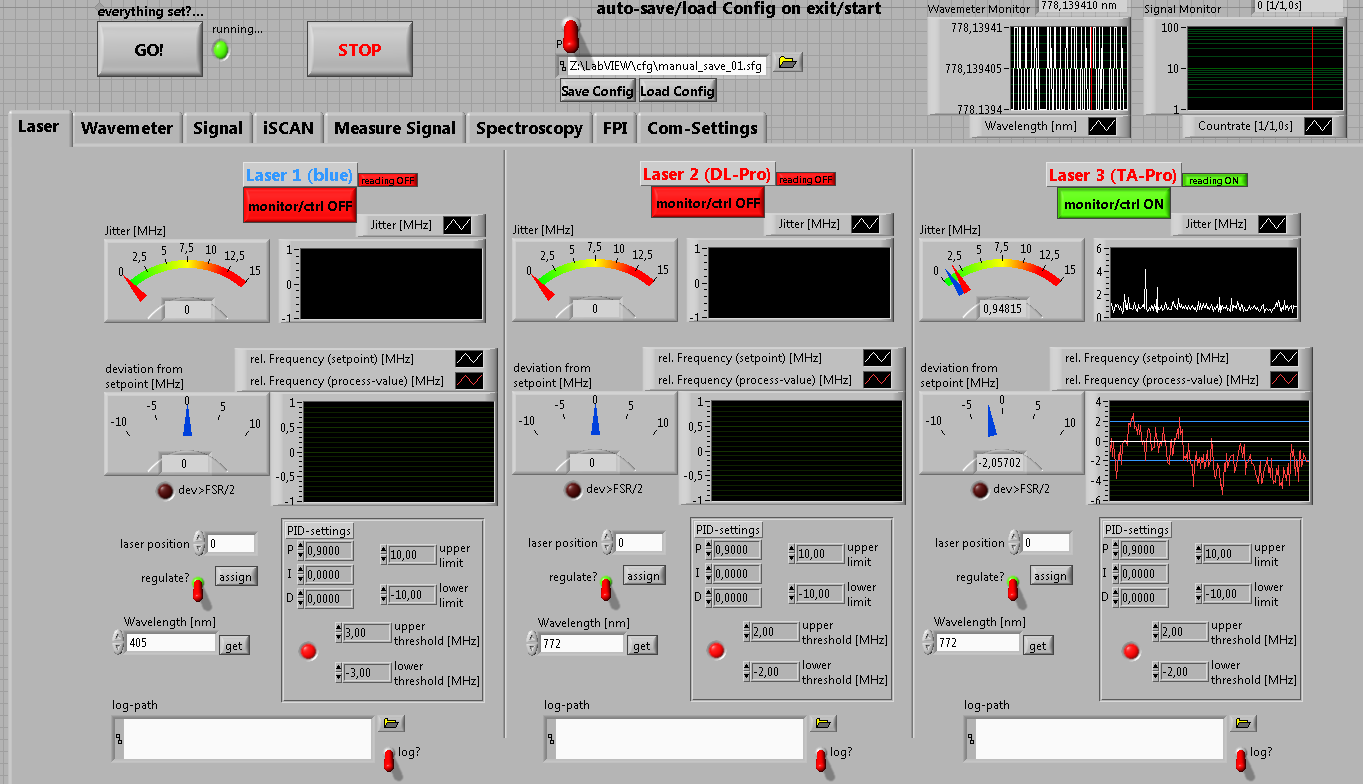
\includegraphics[width=\textwidth-0.5cm]{gfx/benutzeroberflaeche_laserkontrolle}
	    }}
	\caption[Benutzeroberfläche -
	Laserkontrolle]{Bildschirmfoto der Benutzeroberfläche der Laserkontrolle. Laser
	3 ist in Betrieb, die Regelung ist ausgeschaltet.}
	\label{fig:benutzeroberflaeche_laserkontrolle}
\end{figure}

\section{Stabilisierung
und
Frequenzverstimmungsstrategie}\label{sec:stabilisierung_frequenzverstimmungs-strategie}
Frequenzverstimmung und gleichzeitige Regelung wird von der SubVI \lstinline|laser-control.vi| verwaltet. Die Anforderungen sind möglichst schnelles Anfahren der Sollfrequenz, egal, wie groß die Verstimmung ist, und
anschließendes Regeln. Alle im Folgenden verwendeten Frequenzangaben sind
Relativfrequenzen zu einer zu Beginn festgelegten Nullfrequenz. Grundidee ist,
dass der Laser über das \textit{iScan} sehr schnell in den Bereich der
Sollfrequenz gefahren wird und anschließend mithilfe des FOLs nachgeregelt wird,
da ein direktes Anfahren mit dem \textit{iScan} aufgrund seiner Nichtlinearität unmöglich ist. In Kap. \ref{kap:charakterisierung} wird sich zeigen, dass der Fehler bei
alleiniger Verstimmung mit dem \textit{iScan} wenige bis mehr als $100\,$MHz sein kann.
Dies bedarf einer nicht-trivialen Strategie, die mithilfe der Tab.
\ref{tab:scan-strategie_abfolge}, der Abb.
\ref{fig:frequenzverstimmungs-strategie} und des Ablaufdiagramms
\ref{fig:frequenzverstimmungs-strategie_ablaufdiagramm} veranschaulicht werden
soll.\par
\begin{table}
	%Summe der Breiten muss 0.91 mal \textwidth sein.
	\begin{tabular}{p{0.05\textwidth}p{0.86\textwidth}}
		\toprule
			Nr. & Beschreibung \\
		\midrule[1px]
		\hline
			1 & $A\rightarrow B$: Verstimmung in die Mitte des aktuellen FSRs (zwei
			Zwischenschritte mit jeweils anschließender Pause von $17\,$ms)\\
			2 & \textit{Arduino}-FSR-Nummer $n_{Ard,1}$ abfragen\\
			3 & $B\rightarrow C$: großer Zwischenschritt (Vielfaches von FSR)\\
			4 & \textit{Arduino}-FSR-Nummer $n_{Ard,2}$ abfragen\\
			5 & $C\rightarrow D$: Verstimmung um den Rest (drei Zwischenschritte mit
			jeweils anschließender Pause von $17\,$ms)\\
			6 & \textit{Arduino}-FSR-Nummer $n_{Ard,3}$ abfragen\\
		\bottomrule[1px]
	\end{tabular}
	\caption[Laserfrequenzverstimmungs-Strategie]{Zeitliche
	Abfolge der Laserfrequenzverstimmungsstrategie.}
	\label{tab:scan-strategie_abfolge}
\end{table}
\begin{figure}[h]
 	\centering
 	\fbox{\parbox{\dimexpr \linewidth - 2\fboxrule - 2\fboxsep}{
 	\centering
	    
\includegraphics[width=\textwidth-0.5cm]{gfx/frequenzverstimmungs-strategie}
	    }}
	\caption[Frequenzverstimmungs-Strategie]{Frequenzverstimmungs-Strategie,
	im Text näher erklärt.}
	\label{fig:frequenzverstimmungs-strategie}
\end{figure}
%TODO: Fringe A weiter nach links
\begin{figure}[hp]
 	\centering
 	\fbox{\parbox{\dimexpr \linewidth - 2\fboxrule - 2\fboxsep}{
 	\centering
	    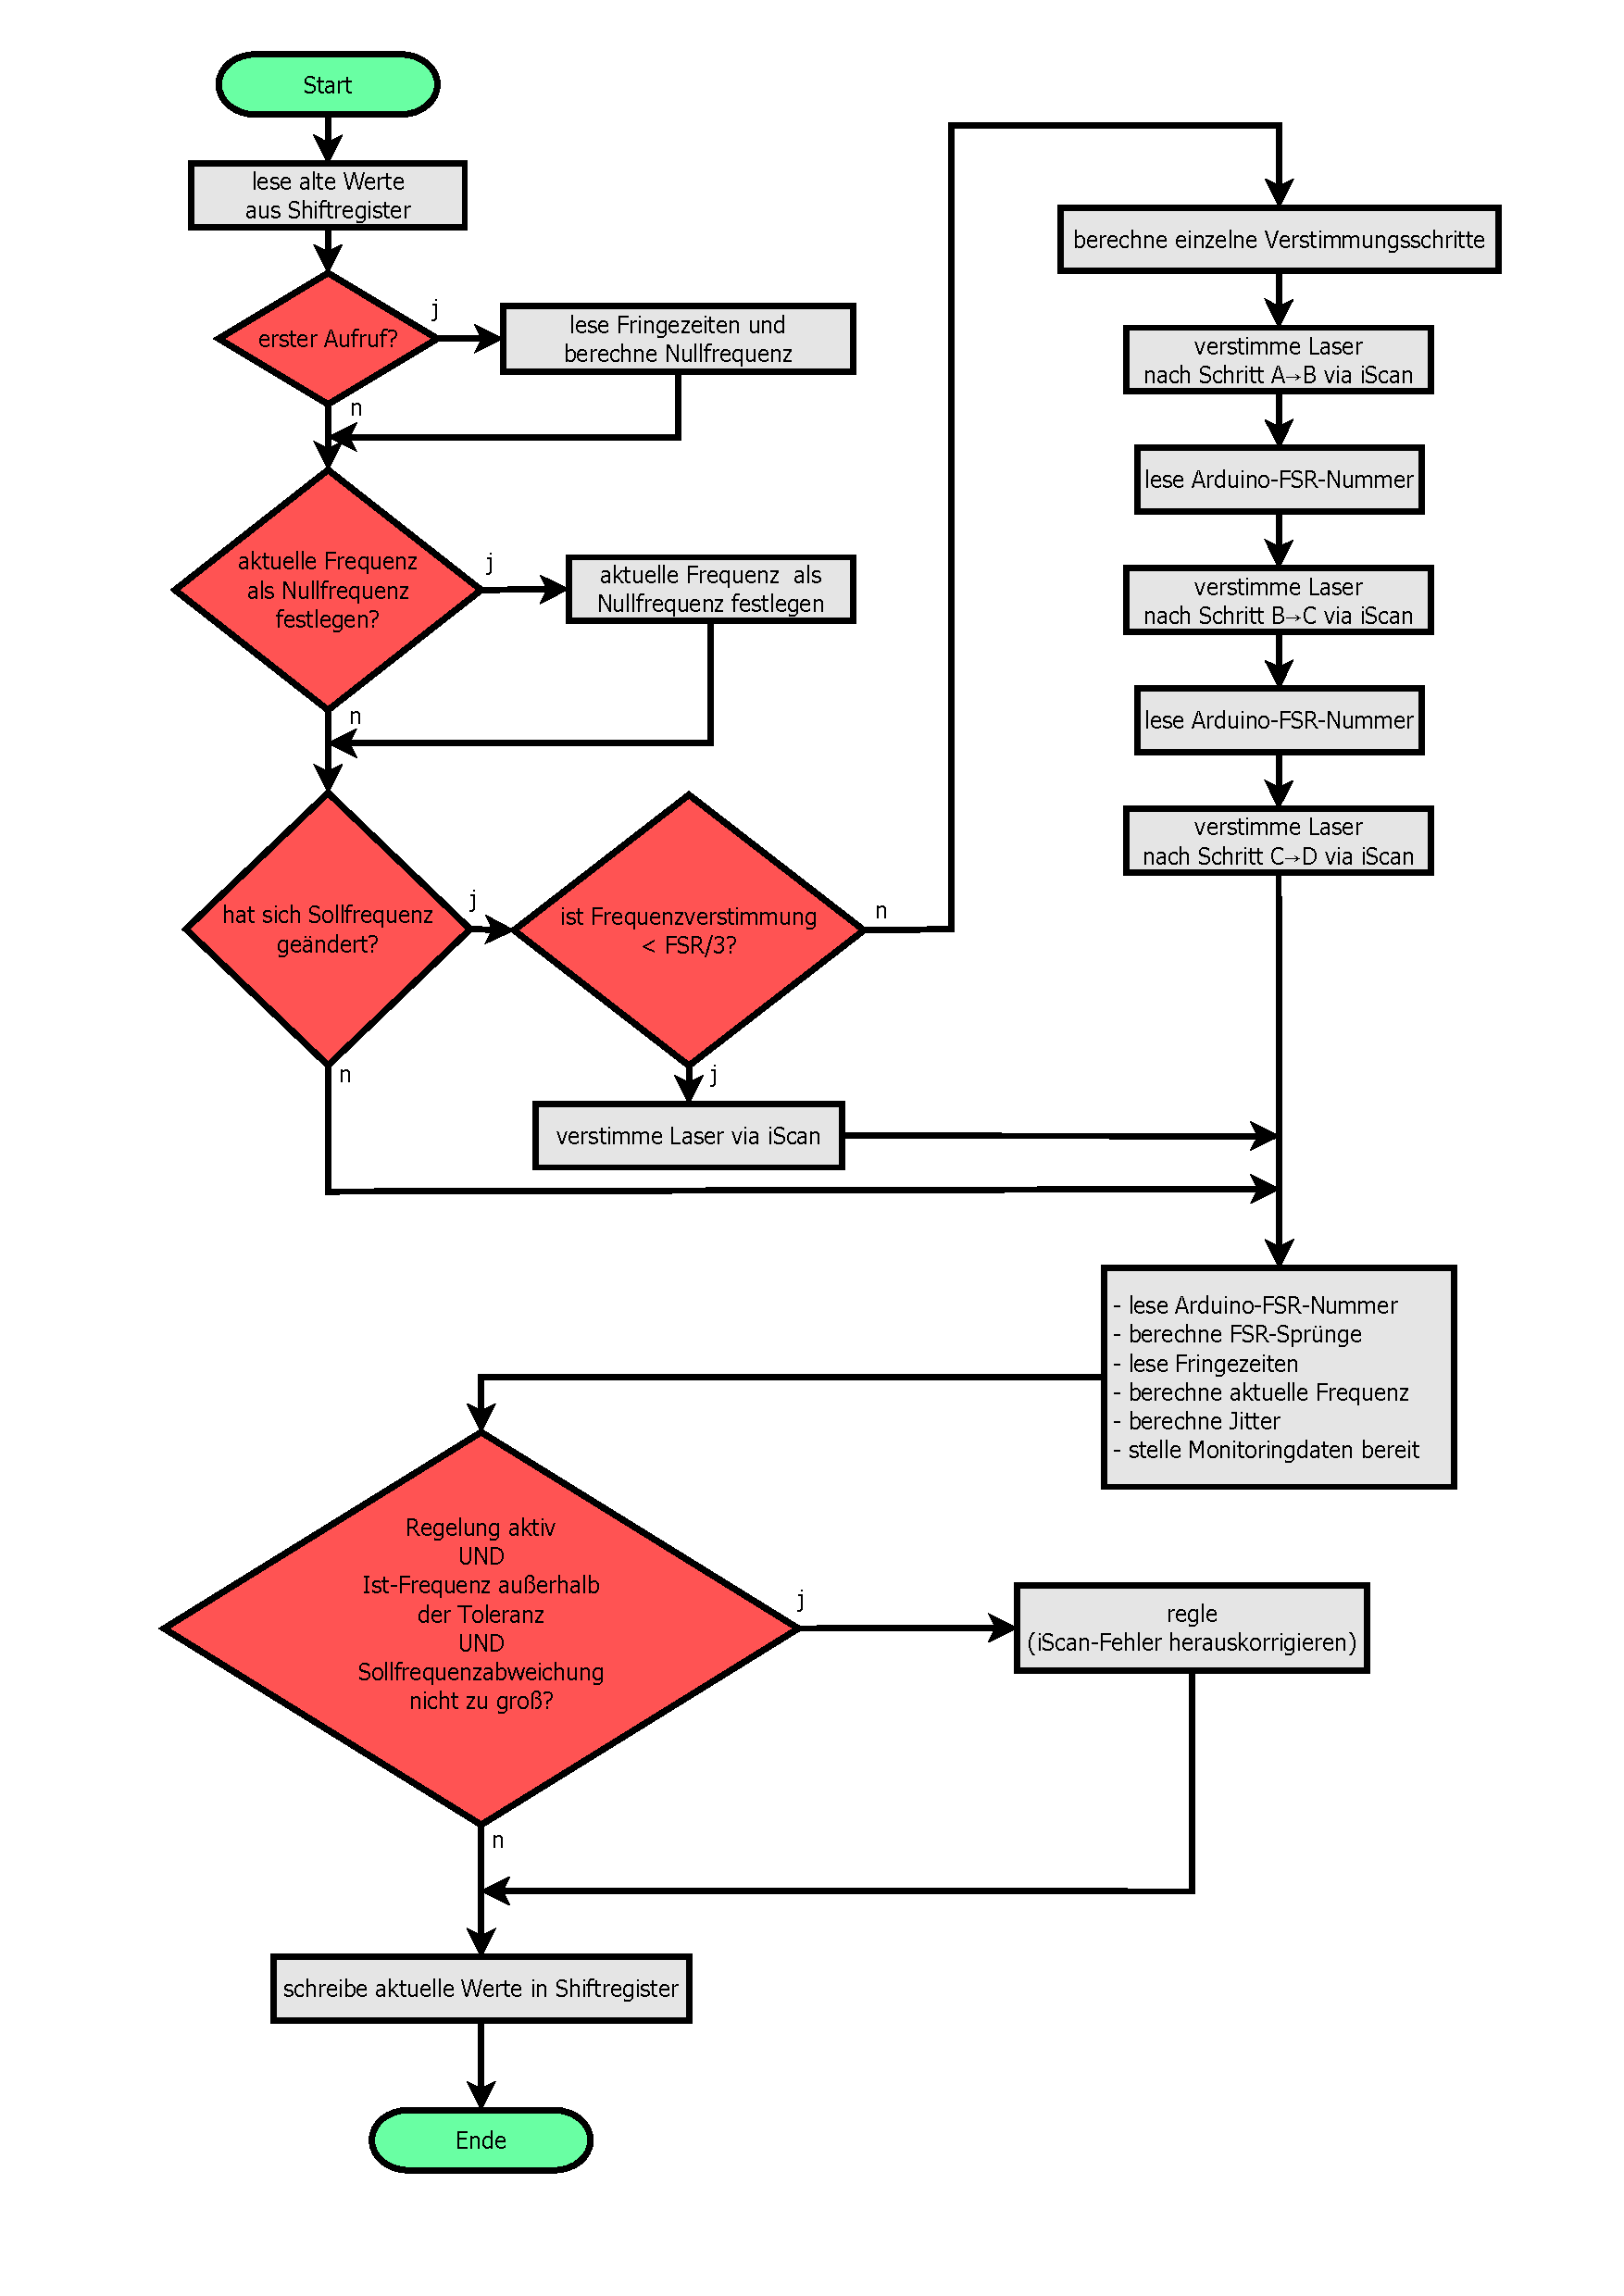
\includegraphics[width=\textwidth-0.5cm]{gfx/frequenzverstimmungs-strategie_ablaufdiagramm}
	    }}
	\caption[Frequenzverstimmungs-Strategie
	-
	Ablaufdiagramm]{Ablaufdiagramm der Frequenzverstimmungs-Strategie, die von der
	SubVI \lstinline|laser-control.vi| implementiert wird. (j=ja, n=nein)}
	\label{fig:frequenzverstimmungs-strategie_ablaufdiagramm}
\end{figure}
Naiverweise könnte man die Strategie verfolgen, den zu verstimmenden
Frequenzwert in ein Vielfaches $n$ des FSRs und einen Rest aufzuteilen. Mit dem
\textit{iScan} würde man den Laser um $n\cdot\text{FSR}$ schnell verfahren,
die aktuelle FSR-Nummer $n_{Ard,1}$ vom \textit{Arduino} auslesen und anschließend
noch die Restfrequenz mit dem \textit{iScan} in drei gleich großen
Schritten\footnote{Der Rest des Verstimmungsvorgangs würde in drei Schritte
aufgeteilt, damit der Laser pro Schritte maximal um $\nicefrac{\text{FSR}}{3}$
verfahren würde.} verfahren. Zwischen jedem Einzelschritt würde $17\,$ms
gewartet werden, damit ein eventueller FSR-Sprung detektiert werden kann.
Nach einem erneuten Abfragen der FSR-Nummer $n_{Ard,2}$ könnte man aus der zu
verstimmenden Frequenz $\Delta\nu$ die erreichte Frequenz über\footnote{$\lfloor x\rfloor$ ist die größt mögliche Ganzzahl n,
für die $n<x$ gilt.}
\begin{equation}\label{eq:neue_frequenz_strategie_1}
	\begin{split}
		\nu_{Ist,nach} &=
		n_{Lab,nach}\cdot\text{FSR}+(\nu_{Offset,nach}-\nu_{Offset,vor})\\
		\text{mit}\quad
		n_{Lab,nach} &= n_{Lab,vor}+n+(n_{Ard,2}-n_{Ard,1})\\
		\text{und}\quad n &=
		\left\lfloor\frac{\Delta\nu}{\text{FSR}}\right\rfloor\,,
	\end{split}
\end{equation} berechnen, wobei $n_{Lab,nach}$ bzw. $n_{Lab,vor}$ die von \textit{Labview}
verwaltete FSR-Nummer und $\nu_{Offset,nach}$ bzw. $\nu_{Offset,vor}$ die
Frequenzposition des Lasers im FSR relativ zum Referenzlaser nach bzw. vor der
Verstimmung sind. Das Nachkorrigieren des \textit{iScan}-Fehlers
$\nu_{Ist}-\nu_{Soll}$ würde dann das FOL übernehmen, das wie in Abschnitt
\ref{sec:iscan_und_fringe-offset-locking} erklärt auch für den Driftausgleich
zuständig ist.\par
Diese Strategie setzt aber eine wichtige und nie sicher gegebene Tatsache
voraus: Bei dem ersten Frequenzverstimmungsschritt $n\cdot\text{FSR}$ geht man
immer davon aus, dass man im $n$-ten FSR des FPIs relativ zur Ausgangsposition
landet. Darauf muss man sich verlassen können, denn eine FSR-Sprung-Detektion
des \textit{Arduinos} ist hier aufgrund des schnellen Verstimmens nicht möglich
und wird schlicht ignoriert. Das Problem hieran ist nun, dass es durchaus vorkommen kann,
wegen des \textit{iScan}-Fehlers nicht im erwarteten FSR zu landen und somit am
Ende einen Fehler von $\pm\text{FSR}$ in der Frequenzberechnung zu erhalten.
Folgende Strategie kann dieses Problem zwar nicht komplett ausschließen, ist aber
wesentlich sicherer, sofern der maximale Verstimmungsfehler des \textit{iScans}
$<\nicefrac{\text{FSR}}{2}$, also ca. $150\,$MHz ist.\par
Die Frequenzverstimmungsmethode besteht aus drei Hauptschritten. Im ersten
Schritt ($A\rightarrow B$) wird der Laser auf eine Frequenz verstimmt, deren
Fringe sich in der Mitte des aktuellen FSRs befindet. Dieser Schritt erfolgt in
zwei gleich großen Teilschritten (maximal $\nicefrac{\text{FSR}}{4}$) mit je
anschließender Pause von $17\,$ms, um sicher FSR-Sprünge detektieren zu können.
Nach einer Abfrage der FSR-Nummer $n_{Ard,1}$ vom \textit{Arduino} folgen zweiter und dritter Schritt ($B\rightarrow C$ und $C\rightarrow D$) analog zur
vorherigen Überlegung (also ein ganzzahliges Vielfaches von FSR im zweiten
Schritt und der Rest im dritten Schritt). Der Fehler im Schritt $B\rightarrow C$
darf also maximal $\nicefrac{\text{FSR}}{2}$ sein, damit der erwartete FSR erreicht wird. Die Verstimmungsfrequenzen der einzelnen Schritte ergeben sich aus
\begin{equation}\label{eq:scan-strategie_schritte}
	\begin{split}
		\Delta\nu_{A\rightarrow B}&=\frac{\text{FSR}}{2}-\nu_{Offset,vor}\\
		\Delta\nu_{B\rightarrow
		C}&=\left\lfloor\frac{(\Delta\nu-\Delta\nu_{A\rightarrow
		B})}{\text{FSR}}\right\rfloor\cdot\text{FSR}\\
		\Delta\nu_{C\rightarrow D}&=(\Delta\nu-\Delta\nu_{A\rightarrow
		B})\mod\text{FSR}\,,
	\end{split}
\end{equation}
wobei $\Delta\nu$ die zu verstimmende Frequenz ist und $\nu_{Offset,vor}$ nicht
relativ zum Referenzlaser, sondern relativ zum Rampenstart gemessen wird. Die
zeitliche Abfolge ist in Tab. \ref{tab:scan-strategie_abfolge} zusammengefasst.
Die erreichte Frequenz berechnet sich dann über
\begin{equation}\label{eq:neue_frequenz_strategie_2}
	\begin{split}
		\nu_{Ist,nach} &=
		n_{Lab,nach}\cdot\text{FSR}+(\nu_{Offset,nach}-\nu_{Offset,vor})\\
		\text{mit}\quad
		n_{Lab,nach} &= n_{Lab,vor}+n+(n_{Ard,1}-n_{Ard,0})+(n_{Ard,3}-n_{Ard,2})\\
		\text{und}\quad
		n &= \left\lfloor\frac{(\Delta\nu-\Delta\nu_{A\rightarrow
		B})}{\text{FSR}}\right\rfloor\,,
	\end{split}
\end{equation}
wobei $n_{Ard,0}$ der \textit{Arduino}-FSR-Nummer $n_{Ard,3}$ des vorherigen
Schleifendurchlaufs der SubVI \lstinline|laser-control.vi| entspricht.\par
Das komplette Ablaufdiagramm des SubVI \lstinline|laser-control.vi| ist in Abb.
\ref{fig:frequenzverstimmungs-strategie_ablaufdiagramm} abgebildet. Dabei ist
der Fall, dass eine neue Soll-Frequenz gesetzt und die oben beschriebene
Rountine abgearbeitet wird, ein spezieller Zweig im Ablauf der SubVI. Genauso
dient das SubVI zum schlichten Festhalten des Lasers. Für die FSR-Berechnung
gilt dann einfach $n=0$ und $n_{Ard,1}=n_{Ard,2}:=n_{Ard,0}$. Gleiches gilt,
wenn der Laser nur um eine Frequenz $<\nicefrac{\text{FSR}}{3}$ verstimmt werden
soll. Ein simples Verstimmen der Laserfrequenz via \textit{iScan} genügt. Um die
Werte am Ende eines Durchlaufs der Routine für den nächsten Schleifendurchlauf
als Eingangswerte zur Verfügung stellen zu können, wird ein Shiftregister
verwendet.
Dieses beinhaltet die in Tab.
\ref{tab:shiftregister_laserkontrolle} aufgeführten Variablen.
\begin{table}
	%Summe der Breiten muss 0.91 mal \textwidth sein.
	\begin{tabular}{p{0.10\textwidth}p{0.81\textwidth}}
		\toprule
			Variable & Beschreibung \\
		\midrule[1px]
		\hline
			$\nu_{Offset}$ & zuletzt gemessene Frequenzposition des Offsetfringes\\
			$\nu_{Offset,ref}$ & Referenzfrequenzposition des Offsetfringes\\
			$\nu_{Soll}$ & momentane Soll-Frequenz relativ zur Nullfreqenz\\
			$\nu_{iScan}$ & Wert des \textit{iScan}-Parameters \lstinline|ScanOffset|\\
			$n_{Lab}$ & zuletzt von \textit{Labview} berechnete FSR-Nummer\\
			$n_{Ard,0,3}$ & zuletzt vom \textit{Arduino} gelieferte FSR-Nummer\\
		\bottomrule[1px]
	\end{tabular}
	\caption[Shiftregister -
	\lstinline|laser-control.vi|]{Shiftregistervariablen der SubVI
	\lstinline|laser-control.vi|.}
	\label{tab:shiftregister_laserkontrolle}
\end{table}
Beim ersten Aufruf der SubVI sind alle Variablen des Shiftregisters außer
$\nu_{iScan}$ null. Bei erneutem Setzen der Nullfrequenz werden $\nu_{Soll}:=0$,
$n_{Lab}:=0$ und $\nu_{Offset,ref}:=\nu_{Offset}$ gesetzt.\par
Nach jedem Durchlauf des SubVI wird eine PID-Regelroutine aufgerufen, welche
nach dem in Abschn. \ref{sec:regeltechnik} erklärten iterativen Verfahren
$\nu_{Ist}$ durch Setzen neuer Werte des
\lstinline|ScanOffset|-Parameters des \textit{iScans} auf $\nu_{Soll}$ regelt.
Dabei können Schwellenwerte für die Regelung (\lstinline|upper threshold| und
\lstinline|lower threshold|) und Maximalregelgrößen (\lstinline|upper limit| und
\lstinline|lower limit|) angegeben werden (siehe Abb.
\ref{fig:benutzeroberflaeche_laserkontrolle}). Mit diesem Verfahren gelingt es,
die Diodenlaser mithilfe der \textit{iScans} sehr schnell (Bruchteile einer
Sekunde) an ihre Sollfrequenzen zu fahren, was sich insbesondere bei
Verstimmungen von mehreren GHz bemerkbar macht. Das Ausgleichen der
\textit{iScan}-Fehler erfolgt allerdings weiterhin langsam. Ziel ist es,
in naher Zukunft die Software performanter zu gestalten, womit mehr
Regelzyklen pro Sekunde abgearbeitet werden können und die insgesamte
Verstimmnungsdauer weniger als eine Sekunde betragen soll.

\section{Linearisierung der \textit{iScans} und
FSR-Korrektur}\label{sec:linearisierung_iscan} Wie schon in den vorigen
Kapiteln erwähnt, muss die Skalierung der \textit{iScans} kalibriert werden.
Diese muss sowohl linear als auch korrekt gestreckt
sein, damit sie sich mit der tatsächlichen Frequenzskala deckt. Um das
Linearitätskriterium zu erfüllen, ist es regelmäßig nötig, die
Phase-Frequenz-Beziehung der LUT der \textit{iScans} zu erneuern. Gleichzeitig
kann auch der FSR des iScans gemessen und ggf. erneuert werden, um die korrekte
Streckung der Skala zu gewährleisten. Ein Maßstab für die Kalibrierung ist der
FSR des FPIs, der bis auf wenige $10\,$kHz genau bestimmt werden kann. Diese
Maßnahmen sorgen für eine Reduktion der Fehler im Verstimmen der Laserfrequenz
mit dem \textit{iScan}. Wie im Abschn.
\ref{sec:stabilisierung_frequenzverstimmungs-strategie} deutlich geworden ist,
sollte der Fehler im ungünstigsten Fall nicht größer als $150\,$MHz sein. Neben
dem Aspekt der Sicherheit in der Frequenzberechnung ist es auch wichtig, den
Fehler des \textit{iScans} mit FOL schnell auszukorrigieren, was eine möglichst
gute Linearität und einen korrekten FSR des \textit{iScans} fordert. Der grobe Ablauf
der Linearisierung wurde bereits in Abschn. \ref{sec:iscan_und_fringe-offset-locking} angerissen. Auf die Stabilisierung des FPIs soll hier nicht weiter eingegangen werden, dazu sei auf das Handbuch des \textit{LaseLock} \cite{laselock} verwiesen.\par
Die \textit{iScan control unit} hat einen analogen Eingang mit
dahintergeschaltetem \textit{Analog-Digital-Converter} (ADC), über den das
Photodiodensignal der FPI-Transmission während eines
Verstimmungsvorgangs digital aufgenommen werden kann. Um eine Repräsentation der
(Nicht-)Linearität der \textit{iScans} zu erhalten, wird eine interne
Frequenzverstimmungsroutine der \textit{iScan control unit} verwendet, die
die Laserfrequenz linear zu den Werten in der LUT durchstimmt.
Durch Auswerten der Distanzen zwischen den einzelnen
Transmissionsfringes in der digitalen Frequenzskala des \textit{iScans} kann
eine Korrektur der LUT-Werte und des digital hinterlegten FSR-Wertes berechnet
werden. Bevor die Verstimmungsroutine starten kann, müssen die in Tab.
\ref{tab:verstimmungsroutine_parameter} aufgelisteten Parameter korrekt
eingestellt werden.
\begin{table}
	%Summe der Breiten muss 0.91 mal \textwidth sein.
	\begin{tabular}{p{0.25\textwidth}p{0.66\textwidth}}
		\toprule
			Parameter & Funktion \\
		\midrule[1px]
		\hline
			\lstinline|ScanOffset| & Startwert der Verstimmungsroutine in MHz\\
			\lstinline|ScanWidth| & Größe des Verstimmungsbereiches in MHz\\
			\lstinline|ScanStepSize| & Schrittweite in MHz\\
			\lstinline|ScanStepDuration| & Wartezeit bis zum nächsten Schritt in ms\\
			\lstinline|Mes_Points| & Anzahl der Schritte (alternativ zu
			\lstinline|ScanStepSize|)\\
			\lstinline|Mes_PointsAuto| & 1: nutze \lstinline|Mes_Points|; 2: nutze
			\lstinline|ScanStepSize|\\
			\lstinline|ScanOnOff| & Verstimmungsroutine aktiv/inaktiv\\
			\lstinline|MeasureScanRuns| & Messroutine aktiv/inaktiv\\
			\lstinline|Measure| & setzt
			\lstinline|MeasureScanRuns=1| und \lstinline|ScanOnOff=1| (Start des Scans
			und Datenaufnahme)\\
		\bottomrule[1px]
	\end{tabular}
	\caption[Parameter der Verstimmungsoutine]{Auswahl der wichtigsten Parameter
	für die Verstimmungsoutine der \textit{iScans}.}
	\label{tab:verstimmungsroutine_parameter}
\end{table}
Alternativ zu \lstinline|ScanStepSize| kann über \lstinline|Mes_Points| die
Anzahl der Schritte angegeben werden, wobei gleichzeitig
\lstinline|Mes_PointsAuto=1| gesetzt sein muss. Über den Parameter
\lstinline|Scn_In[i] = [Input-Kanalnummer]| können 8
verschiedene Datenquellen festgelegt werden, wobei
\lstinline|i| von 0 bis 7 geht und \lstinline|Input-Kanalnummer| die Quelle
der Daten ist. Für den analogen Eingang des ADC ist dies die Kanalnummer 448.
Nach Start der Routine sendet die \textit{iScan scan control unit} zeilenweise
die aktuelle Relativfrequenz und den ADC-Wert. Im Folgenden und mithilfe von
Abb. \ref{fig:linearisierung_ablaufdiagramm} soll nun der Ablauf einer
Linearisierungsroutine für ein einzelnes \textit{iScan}-System erklärt werden.
Die Software baut auf einer von \textit{TEM-Messtechnik} zur Verfügung gestellten
SubVI auf, wobei die Linearisierungsroutine bereits weitgehend implementiert
war. Die Kalibrierung des Parameters \lstinline|FSR| (vermuteter FSR des
\textit{iScans}) wurde nachträglich hinzugefügt.\par
\begin{figure}[hp]
 	\centering
 	\fbox{\parbox{\dimexpr \linewidth - 2\fboxrule - 2\fboxsep}{
 	\centering
	    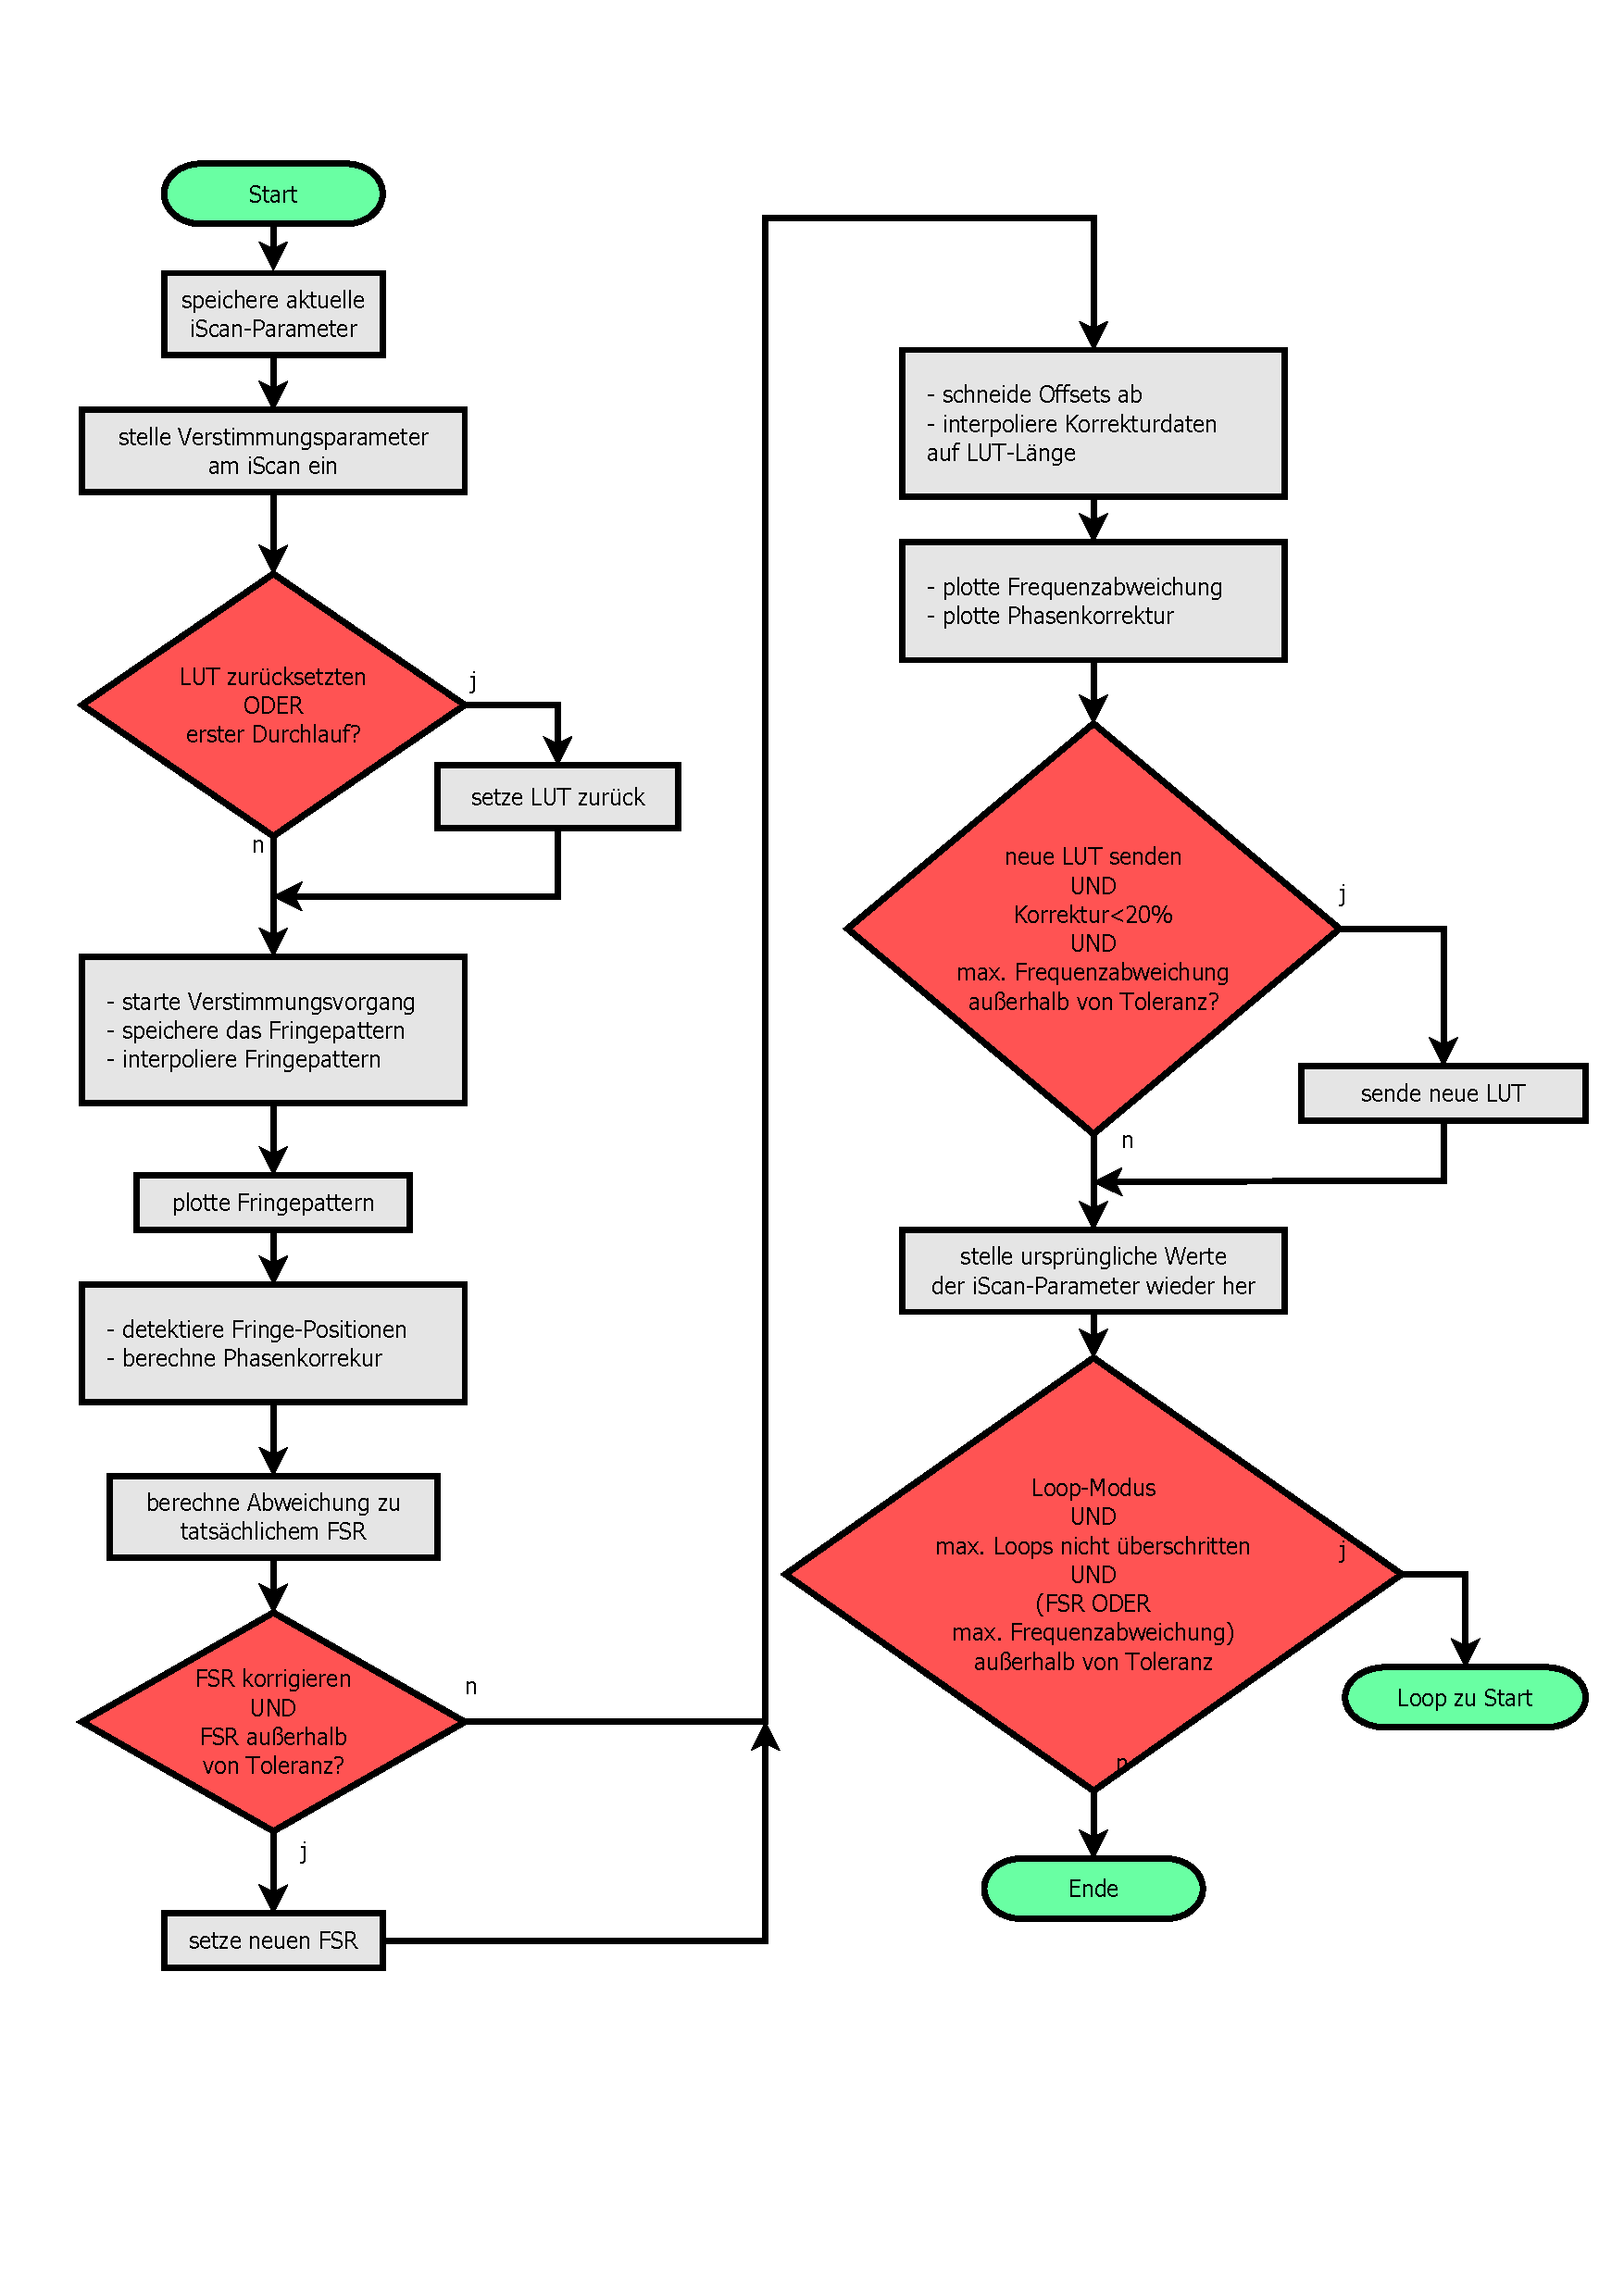
\includegraphics[width=\textwidth-0.5cm]{gfx/linearisierung_ablaufdiagramm}
	    }}
	\caption[Linearisierung der \textit{iScans} -
	Ablaufdiagramm]{Ablaufdiagramm der Linearisierungsroutine
	der \textit{iScans}. (j=ja, n=nein)}
	\label{fig:linearisierung_ablaufdiagramm}
\end{figure}
Zunächst werden alle relevanten aktuellen \textit{iScan}-Parameter
zwischengespeichert, damit sie am Ende der Routine wieder zurückgeschrieben
werden können. Über welchen Frequenzbereich das Fringepattern abgefahren wird,
legt der Parameter \lstinline|FSR| fest.
Prozentual zu \lstinline|FSR| wird ein Offset berechnet, mit dem der abzufahrende Frequenzbereich erweitert wird, damit
Nichtlinearitäten am Anfang und am Ende des Bereichs abgeschnitten werden
können. Beim ersten Durchlauf der Lineariseirungsroutine wird die LUT
zurückgesetzt. Das bedeutet, sie wird mit Werten $A_i$ und $B_i$ gefüllt, die
die äquidistanten Punkte auf einem Kreis repräsentieren. Sind alle nötigen
Parameter gesetzt, beginnt das Abfahren der Frequenz linear zur LUT, wobei die
Messwerte des Fringepattern und die Frequenzwerte parallel in ein Array
gespeichert werden. Das Fringepattern wird auf der
Benutzeroberfläche angezeigt (siehe
\ref{fig:linearisierung_benutzeroberflaeche_fringepattern}).\par
\begin{figure}[h]
 	\centering
 	\fbox{\parbox{\dimexpr \linewidth - 2\fboxrule - 2\fboxsep}{
 	\centering
	    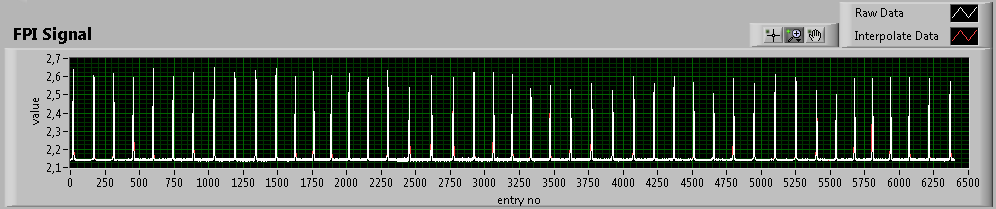
\includegraphics[width=\textwidth-0.5cm]{gfx/linearisierung_benutzeroberflaeche_fringepattern}
	    }}
	\caption[Benutzeroberfläche Linearisierung -
	Fringepattern]{Bildschirmfoto der Ausgabe des Fringepatterns und dessen
	Interpolation auf der Benutzeroberfläche. \textit{entry no} ist die Stelle
	eines jeden Elements des Datenarrays (Verstimmungsschritt). Die Schrittweite
	der Frequenzverstimmung war hier $2\,$MHz.}
	\label{fig:linearisierung_benutzeroberflaeche_fringepattern}
\end{figure}
Je nach eingestellter Schrittweite und Verweilzeit pro Schritt kann die
Aufnahme des Fringepatter $30\,$s bis $1\,$min dauern. Vor der
Weiterverarbeitung des Fringepattern wird dieses zur Glättung mehrfach interpoliert, damit es keine Probleme bei der Positionsbestimmung der Fringes
gibt. Das interpolierte Fringepattern wird nun in ein
geschütztes\footnote{Quelltext nicht offen} SubVI von \textit{TEM-Messtechnik} gegeben, das die Fringepositionen detektiert, die Frequenzabstände der Fringes
untereinander analysiert und ein Array mit der aktuellen Phasenabweichung von
der Linearität ausgibt. Anschließend wird das Array negiert, dessen Offsets
abgeschnitten und auf die Länge $N$ der LUT-Tabelle interpoliert, sodass sich
$N$ Phasenkorrekturwerte $\Delta\phi_i$ im Intervall
$[0,\text{\lstinline|FSR|})$ ergeben. Die neuen LUT-Einträge
\begin{equation}\label{eq:LUT_korrektur_01}
	\begin{split}
		A_i&=-A\cdot\cos{\left(2\pi\frac{i}{N}+\Delta\phi_i\right)}\\
		&\text{und}\\
		B_i&=B\cdot\sin{\left(2\pi\frac{i}{N}+\Delta\phi_i\right)}\,.
	\end{split}
\end{equation}
werden durch Modulation einer Kreisquadratur mit der Phasenkorrektur
berechnet und in die LUT-Tabelle geschrieben. Ist die
maximale Frequenzabweichung nach der Korrektur nicht unter einem vom Benutzer
frei wählbaren Toleranzwert, wird die Routine ein weiteres Mal durchlaufen,
wobei die LUT eingangs nicht mehr zurückgesetzt wird. Stattdessen werden die neuen Korrekturwerte über
\begin{equation}\label{eq:LUT_korrektur_02}
	\Delta\phi_i=\Delta\phi_{i,alt}-\Delta\phi_{i,akt}
\end{equation}
berechnet, wobei $\Delta\phi_{i,alt}$ die Korrekturwerte $\Delta\phi_i$
des vorherigen Durchlaufs und $\Delta\phi_{i,akt}$ die aktuellen Korrekturwerte
sind. Die Aufnahme des Fringepattern und die Phasenkorrektur wiederholen sich so
lange, bis der Toleranzwert unterschritten wurde. Abbildung
\ref{fig:linearisierung_benutzeroberflaeche_phasenkorrektur} zeigt die Ausgabe der Phasenkorrektur auf der Benutzeroberfläche mit eingangs zurückgesetzter LUT.\par
\begin{figure}[h]
 	\centering
 	\fbox{\parbox{\dimexpr \linewidth - 2\fboxrule - 2\fboxsep}{
 	\centering
	    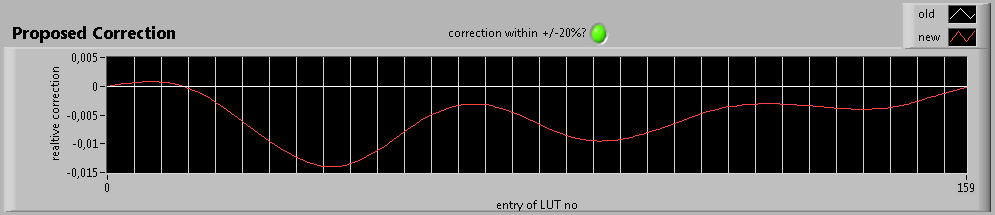
\includegraphics[width=\textwidth-0.5cm]{gfx/linearisierung_benutzeroberflaeche_phasenkorrektur}
	    }}
	\caption[Benutzeroberfläche Linearisierung -
	Phasenkorrektur]{Bildschirmfoto der Ausgabe der Phasenkorrekturwerte auf der
	Benutzeroberfläche nach erstmaligem Linearisieren. \textit{entry
	of LUT no} ist die Nummer des Zeileneintrags in der LUT. \textit{relative
	correction} ist die relative Phasenkorrektur des jeweiligen Eintrags. Dabei
	entspricht 1 dem vollen Kreis, also $2\pi$. Der weiße Plot beschreibt die
	vorige Linearitätskorrektur (hier konstant 0, da die LUT eingangs zurückgesetzt
	wurde). Der rote Plot beschreibt die Korrektur nach Messen der neuen
	Linearitätsabweichung.}
	\label{fig:linearisierung_benutzeroberflaeche_phasenkorrektur}
\end{figure}
%TODO: Plots dicker
Neben der Linearität der \textit{iScans} kann auch die Korrektur des Parameters
\lstinline|FSR| bestimmt werden. Dazu betrachtet man zunächst die
Abweichung der \textit{iScan}-Skala zur tatsächlichen Frequenz. In
\ref{fig:linearisierung_benutzeroberflaeche_frequenz-abweichung} ist die
Ausgabe der Abweichung auf der Benutzeroberfläche dargestellt.
\begin{figure}[h]
 	\centering
 	\fbox{\parbox{\dimexpr \linewidth - 2\fboxrule - 2\fboxsep}{
 	\centering
	    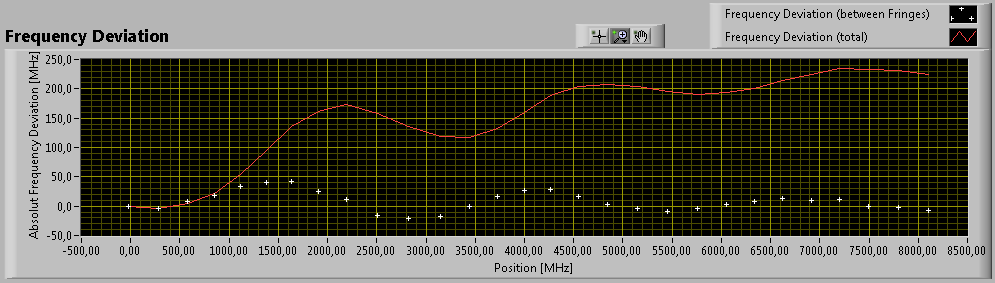
\includegraphics[width=\textwidth-0.5cm]{gfx/linearisierung_benutzeroberflaeche_frequenz-abweichung}
	    }}
	\caption[Benutzeroberfläche Linearisierung -
	Frequenzfehler]{Bildschirmfoto der Ausgabe des Frequenzfehlers
	auf der Benutzeroberfläche. Die weißen Punkte sind die einzelnen Abweichungen
	der Frequenzabstände benachbarter Fringes zum FSR des FPIs. Der rote Plot ist
	die totale Frequenzabweichung realtiv zur ersten Fringeposition.}
	\label{fig:linearisierung_benutzeroberflaeche_frequenz-abweichung}
\end{figure}
Die weißen Punkte stellen die Abweichung der einzelnen Nachbarfringeabstände zum
FSR des FPIs dar. Die rote Kurve beschreibt den absoluten Fehler des
\textit{iScans} bezogen auf die erste Fringeposition. Verschwindet die
Differenz zwischen dem Offset der Kurve bei $\nu=0$ und dem Offset bei
$\nu=\text{\lstinline|FSR|}$, kann man davon ausgehen, dass der Parameter
\lstinline|FSR| auch den tatsächlichen FSR des \textit{iScans} repräsentiert.
Ist der Fehler allerdings $>0$ bzw. $<0$, so
ist der Parameter \lstinline|FSR| zu klein bzw. zu groß gewählt und muss
ensprechend nachkorrigiert werden.\par
Problem bei der Berechnung der Abweichung
zum wahren Wert des FSRs ist, dass nur diskrete Messpunkte im Frequenzabstand
von einem FPI-FSR, also ca. $300\,$MHz vorliegen. Eine Möglichkeit ist, nach
erfolgreicher Linearisierung einen linearen Fit der totalen Frequenzabweichung
zu machen. Die Differenz der Offsets bei $\nu=0$ und
$\nu=\text{\lstinline|FSR|}$ ergibt dann den Korrekturwert. Eine genauere und
linearisierungsunabhängige Methode, die hier implementiert wurde, soll im
Folgenden kurz erläutert werden.\par
\begin{figure}[h]
 	\centering
 	\fbox{\parbox{\dimexpr \linewidth - 2\fboxrule - 2\fboxsep}{
 	\centering
	    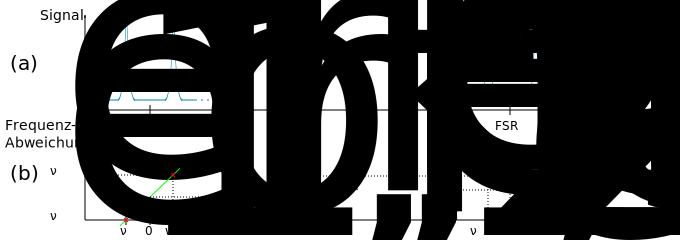
\includegraphics[width=\textwidth-0.5cm]{gfx/FSR-korrektur}
	    }}
	\caption[\textit{iScan}-FSR-Korrektur -
	Methode]{Methode zur Korrektur des \text{iScan}-FSRs. In (a) ist Anfang und
	Ende des Fringepattern zu sehen. (b) zeigt die zur FSR-Korrektur nötigen
	Größen. Dabei ist $\text{FSR}_{est}$ der angegebene FSR des \textit{iScans}
	(Parameter \lstinline|FSR|) und $\text{FSR}_{korr}$ der Korrekturwert.}
	\label{fig:FSR-korrektur}
\end{figure}
%TODO: !mit dem Screenshot in ein Bild mit subfloats; außerdem größer
Zur Berechnung werden die zwei Messpunkte der totalen Abweichung jeweils vor und
nach $\nu=0$ bzw. $\nu=\text{\lstinline|FSR|}$ benötigt ($\nu_{i,j}$ und
$\nu_{err,i,j}$ in Abb. \ref{fig:FSR-korrektur}(b)). Es ist nur von Interesse,
wie groß die Aweichungen bei $\nu=0$ und $\nu=\text{\lstinline|FSR|}$ sind. Die Abweichung dazwischen ist
unerheblich, womit unabhängig von der Linearisierung eine FSR-Korrektur
durchgeführt werden kann. Es werden nun jeweils lineare Fits einmal durch die
beiden Punkte $(\left.\nu_{1,1}\right|\nu_{err,1,1})$ und
$(\left.\nu_{1,2}\right|\nu_{err,1,2})$ und einmal durch die Punkte
$(\left.\nu_{2,1}\right|\nu_{err,2,1})$ und
$(\left.\nu_{2,2}\right|\nu_{err,2,2})$ gelegt.
Die Differenz der Offsets der Schnittpunkte der Geraden bei $\nu=0$ und
$\nu=\text{\lstinline|FSR|}$ ergeben den Wert für die FSR-Korrektur:
\begin{equation}\label{eq:FSR_korrektur}
	\begin{split}
		\text{FSR}_{korr}
		&=\nu_{offs,2}-\nu_{offs,1}\\
		&=a_2(\text{\lstinline|FSR|}-\nu_{2,1})+\nu_{err,2,1}-[a_1(-\nu_{1,1})+\nu_{err,1,1}]\\
		&=\frac{\nu_{err,2,2}-\nu_{err,2,1}}{\nu_{2,2}-\nu_{2,1}}(\text{\lstinline|FSR|}-\nu_{2,1})+\nu_{err,2,1}+\frac{\nu_{err,1,2}-\nu_{err,1,1}}{\nu_{1,2}-\nu_{1,1}}\nu_{1,1}-\nu_{err,1,1}\,.
	\end{split}
\end{equation}
Im Beispiel \ref{fig:linearisierung_benutzeroberflaeche_frequenz-abweichung}
ist $\text{FSR}_{korr}=238,6\,$MHz. Es wurde ein FSR von $8000\,$MHz angenommen,
also $\text{\lstinline|FSR|}=\text{FSR}_{est}=8000\,$MHz. Nach der Korrektur
würde gelten $\text{\lstinline|FSR|}=\text{FSR}_{est,neu}=8239\,$MHz
(Rundung auf Ganzzahl).\par
Neben der Linearisierung und der FSR-Korrektur der
\textit{iScans} bietet die Routine auch ein schlichtes Überwachen der Linearität
und des FSRs. Dazu werden die Korrekturfunktionen einfach abgeschaltet.

\section{Experimentsteuerung}\label{sec:experimentsteuerung}
In diesem Abschnitt wird der Teil der Software behandelt, der für die Steuerung
des Experiments und die Aufnahme der Messdaten verantwortlich ist. In Abschn.
\ref{subsec:messdatenerfassung} soll die softwareseitige Datenaufnahme kurz
beschrieben werden. Abschnitt \ref{subsec:spektroskopie_software} befasst sich mit den
Funktionen, die die Möglichkeit bieten spektroskopische Untersuchungen
weitgehendst automatisch durchzuführen.\par
Neben diesen Funktionen ist in naher Zukunft noch die Implementierung von
Erweiterungen vorgesehen. Es soll eine Steuerung des QMS nachgerüstet werden, um
Massenscans durchführen zu können. Auch eine Ofensteuerung ist optional geplant.
Darüber hinaus soll eine automatisierte Routine für Isotopenverhältnismessungen
programmiert werden. Da der Schwerpunkt dieser Arbeit auf der Entwicklung des
Lasersystems und dessen Charakterisierung liegt, wurden zunächst nur die dafür
nötigen Funktionen implementiert.

\subsection{Messdatenerfassung}\label{subsec:messdatenerfassung}
Zu den bisher nötigen Messdaten zählen die Absolutwellenlänge des Wavemeters und
die Countrate des Channeltrons. Beide Werte erreichen den PC via RS232 als
Gleitkomma- bzw. Dezimalwerte. Analog zu den Laserdaten des FOL werden diese
Werte zur Vermeidung eines Pufferstaus direkt in jeweilige globale Variablen
geschrieben und mit einem boolschen Wert versehen, der angibt, ob die Werte
aktuell oder schon gelesen worden sind. Auch hier liegt die Priorität auf der
Aktualität der Daten und nicht darauf, jeden Wert zu erfassen. Beide Werte
können über die SubVIs \lstinline|get_wavemeter_data.vi| und
\lstinline|get_countrate_data.vi| aus den globalen Variablen ausgelesen
werden.\par
Die Wellenlänge wird mit dem Wavemeter gemessen, dessen Software auf einem
separaten PC läuft. Sie schickt in regelmäßigen Abständen die Wellenlänge in nm
(Vakuumwellenlänge) seriell an den PC, auf dem das \textit{Labview}-Programm läuft. Die Daten für die Countrate werden wie schon
erwähnt von einem \textit{Arduino} aufbereitet und ebenso an
den PC geschickt. Der Quelltext des Programms für den \textit{Arduino} ist in Anh.
\ref{anh:sec:quelltext_arduino_countrate} einzusehen.\par
Sowohl die Wellenlänge/Frequenz/Wellenzahl als auch die Countrate kann
permanent auf der Benutzeroberfläche überwacht werden. Weiterhin können die
Wiederholraten der Anzeigen angegeben und das zeitliche Verhalten der Messdaten
aufgezeichnet werden.

\subsection{Spektroskopie}\label{subsec:spektroskopie_software}
Um atomare Übergänge zu finden und zu charakterisieren ist es nötig, Countraten
gegen Frequenz aufzunehmen. Abbildung \ref{fig:spektroskopie_benutzeroberflaeche}
zeigt die Benutzeroberfläche des \textit{Labview}-Programmteils zur
Spektroskopie.
\begin{figure}[h]
 	\centering
 	\fbox{\parbox{\dimexpr \linewidth - 2\fboxrule - 2\fboxsep}{
 	\subfloat[]{
		\label{subfig:spektroskopie_benutzeroberflaeche_manuell}
		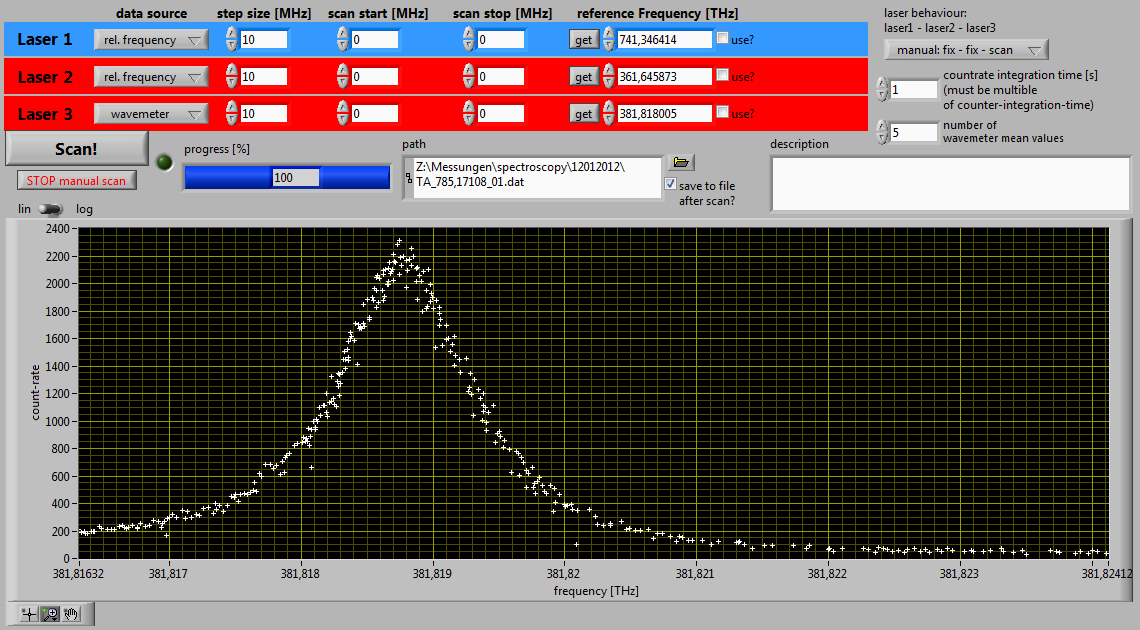
\includegraphics[width=\textwidth-0.4cm]{gfx/spektroskopie_benutzeroberflaeche_manuell}
		}\\
	\subfloat[]{
		\label{subfig:spektroskopie_benutzeroberflaeche_automatisch}
		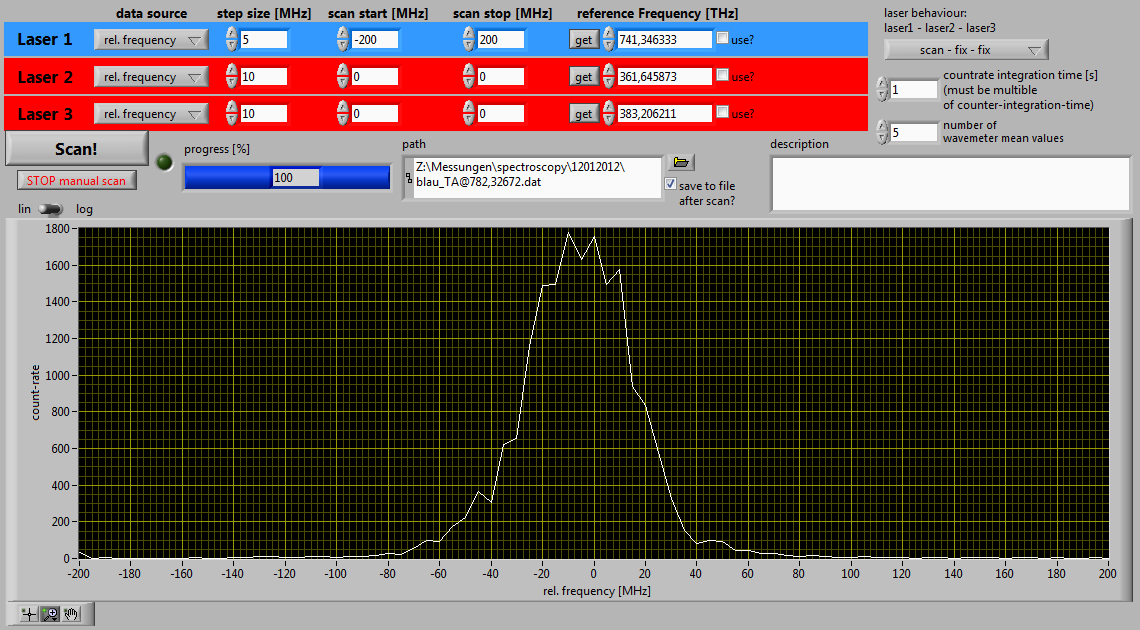
\includegraphics[width=\textwidth-0.4cm]{gfx/spektroskopie_benutzeroberflaeche_automatisch}
		}
	}}
	\caption[Benutzeroberfläche
	Spektroskopie]{Benutzeroberfläche für Spektroskopiemessungen mit
	eindimensionalen Scans. In (a) ist ein manueller Scan zu sehen, wobei Laser 1
	und 2 auf ihrer Frequenz festgehalten wurden und Laser 3 manuell mit dem
	\textit{iScan} verstimmt wurde. (b) zeigt einen automatischen Scan, bei dem die
	Frequenzen der Laser 2 und 3 stabilisiert und festgehalten und Laser 1
	automatisch vertsimmt wurde.}
	\label{fig:spektroskopie_benutzeroberflaeche}
\end{figure}
Im Folgenden sollen zunächst alle Funktionen beschrieben und
anschließend der Ablauf eines Messvorgangs erklärt werden.\par
Es ist möglich, sowohl \textit{eindimensionale Scans} als auch
\textit{mehrdimensionale Scans} durchzuführen. Unter eindimensionalen Scans
versteht man die Countratenaufnahme beim Verstimmen der Frequenz eines Lasers
und Festhalten der Frequenzen der anderen beiden Laser. Bei zwei- bzw.
dreidimensionalen Scans wird ein zwei- bzw. dreidimensionales Frequenzraster von
zwei bzw. allen drei Lasern abgetastet. Dabei wird die Frequenz des Laser in der
ersten Dimension permanent von Start bis Ende durchgefahren und nach jedem
Durchlauf die Frequenz des Lasers der nächsthöheren Dimension auf den nächsten
Frequenzschritt eingestellt. Unter \textit{laser behaviour} kann zwischen
allen möglichen Kombinationen, die sich dadurch ergeben, entschieden werden.
Weiterhin wird im eindimensionalen Fall angeboten, die Laserfrequenz manuell zu
verstimmen (beispielsweise durch manuelles
Ändern des Parameters \lstinline|ScanOffset| des \textit{iScans}, 
vorausgesetzt FOL ist deaktiviert).\par
Als Frequenzdatenquelle kann unter \textit{data
source} zwischen der Relativfrequenz gemäß
$\nu_{Soll}$ aus Abschn. \ref{sec:stabilisierung_frequenzverstimmungs-strategie}
und der Absolutfrequenz über das Wavemeter gewählt werden. Selbstverständlich
kann immer nur für einen Laser das Wavemeter als Datenquelle dienen. Ein Scan ist immer in
diskrete Frequenzschritte mit der maximalen Auflösung von $1\,$MHz unterteilt
(\textit{step size}). Soll ein Scan automatisch erfolgen, muss für die zu
verstimmende(n) Laserfrequenz(en) ein Start- und ein Stopwert angegeben werden.
Werden Relativfrequenzen aufgenommen, ist es immer sinnvoll eine absolute
Frequenz als Referenz zu haben. Dazu kann über den Button \textit{get} die
Absolutfrequenz des Lasers aus dem Wavemeter ausgelesen werden. Mit
\textit{use?} kann entschieden werden, ob die Absolutfrequenz beim Abspeichern
der Werte auf die Relativfrequenz addiert werden soll. In jedem Fall wird die
Absolutfrequenz in den Header der Aufnahmedatei gespeichert.\par
Weiterhin kann die Integrationszeit für die Countrate ausgewählt und die Anzahl
der Wavemeter-Werte, die gemittelt werden sollen, angegeben werden. Da das
Wavemeter ab und zu fälschlicherweise Werte in völlig anderen
Wellenlängenbereichen detektiert (Einflüsse der Multimode-Glasfaser), wurde bei
der Mittelung darauf geachtet, unplausible Werte zu ignorieren.\par
Abbildung \ref{fig:spektroskopie_ablaufdiagramm} veranschaulicht noch einmal
schematisch den allgemeinen Ablauf eines Frequenzscans.
\begin{figure}[hp]
 	\centering
 	\fbox{\parbox{\dimexpr \linewidth - 2\fboxrule - 2\fboxsep}{
 	\centering
	    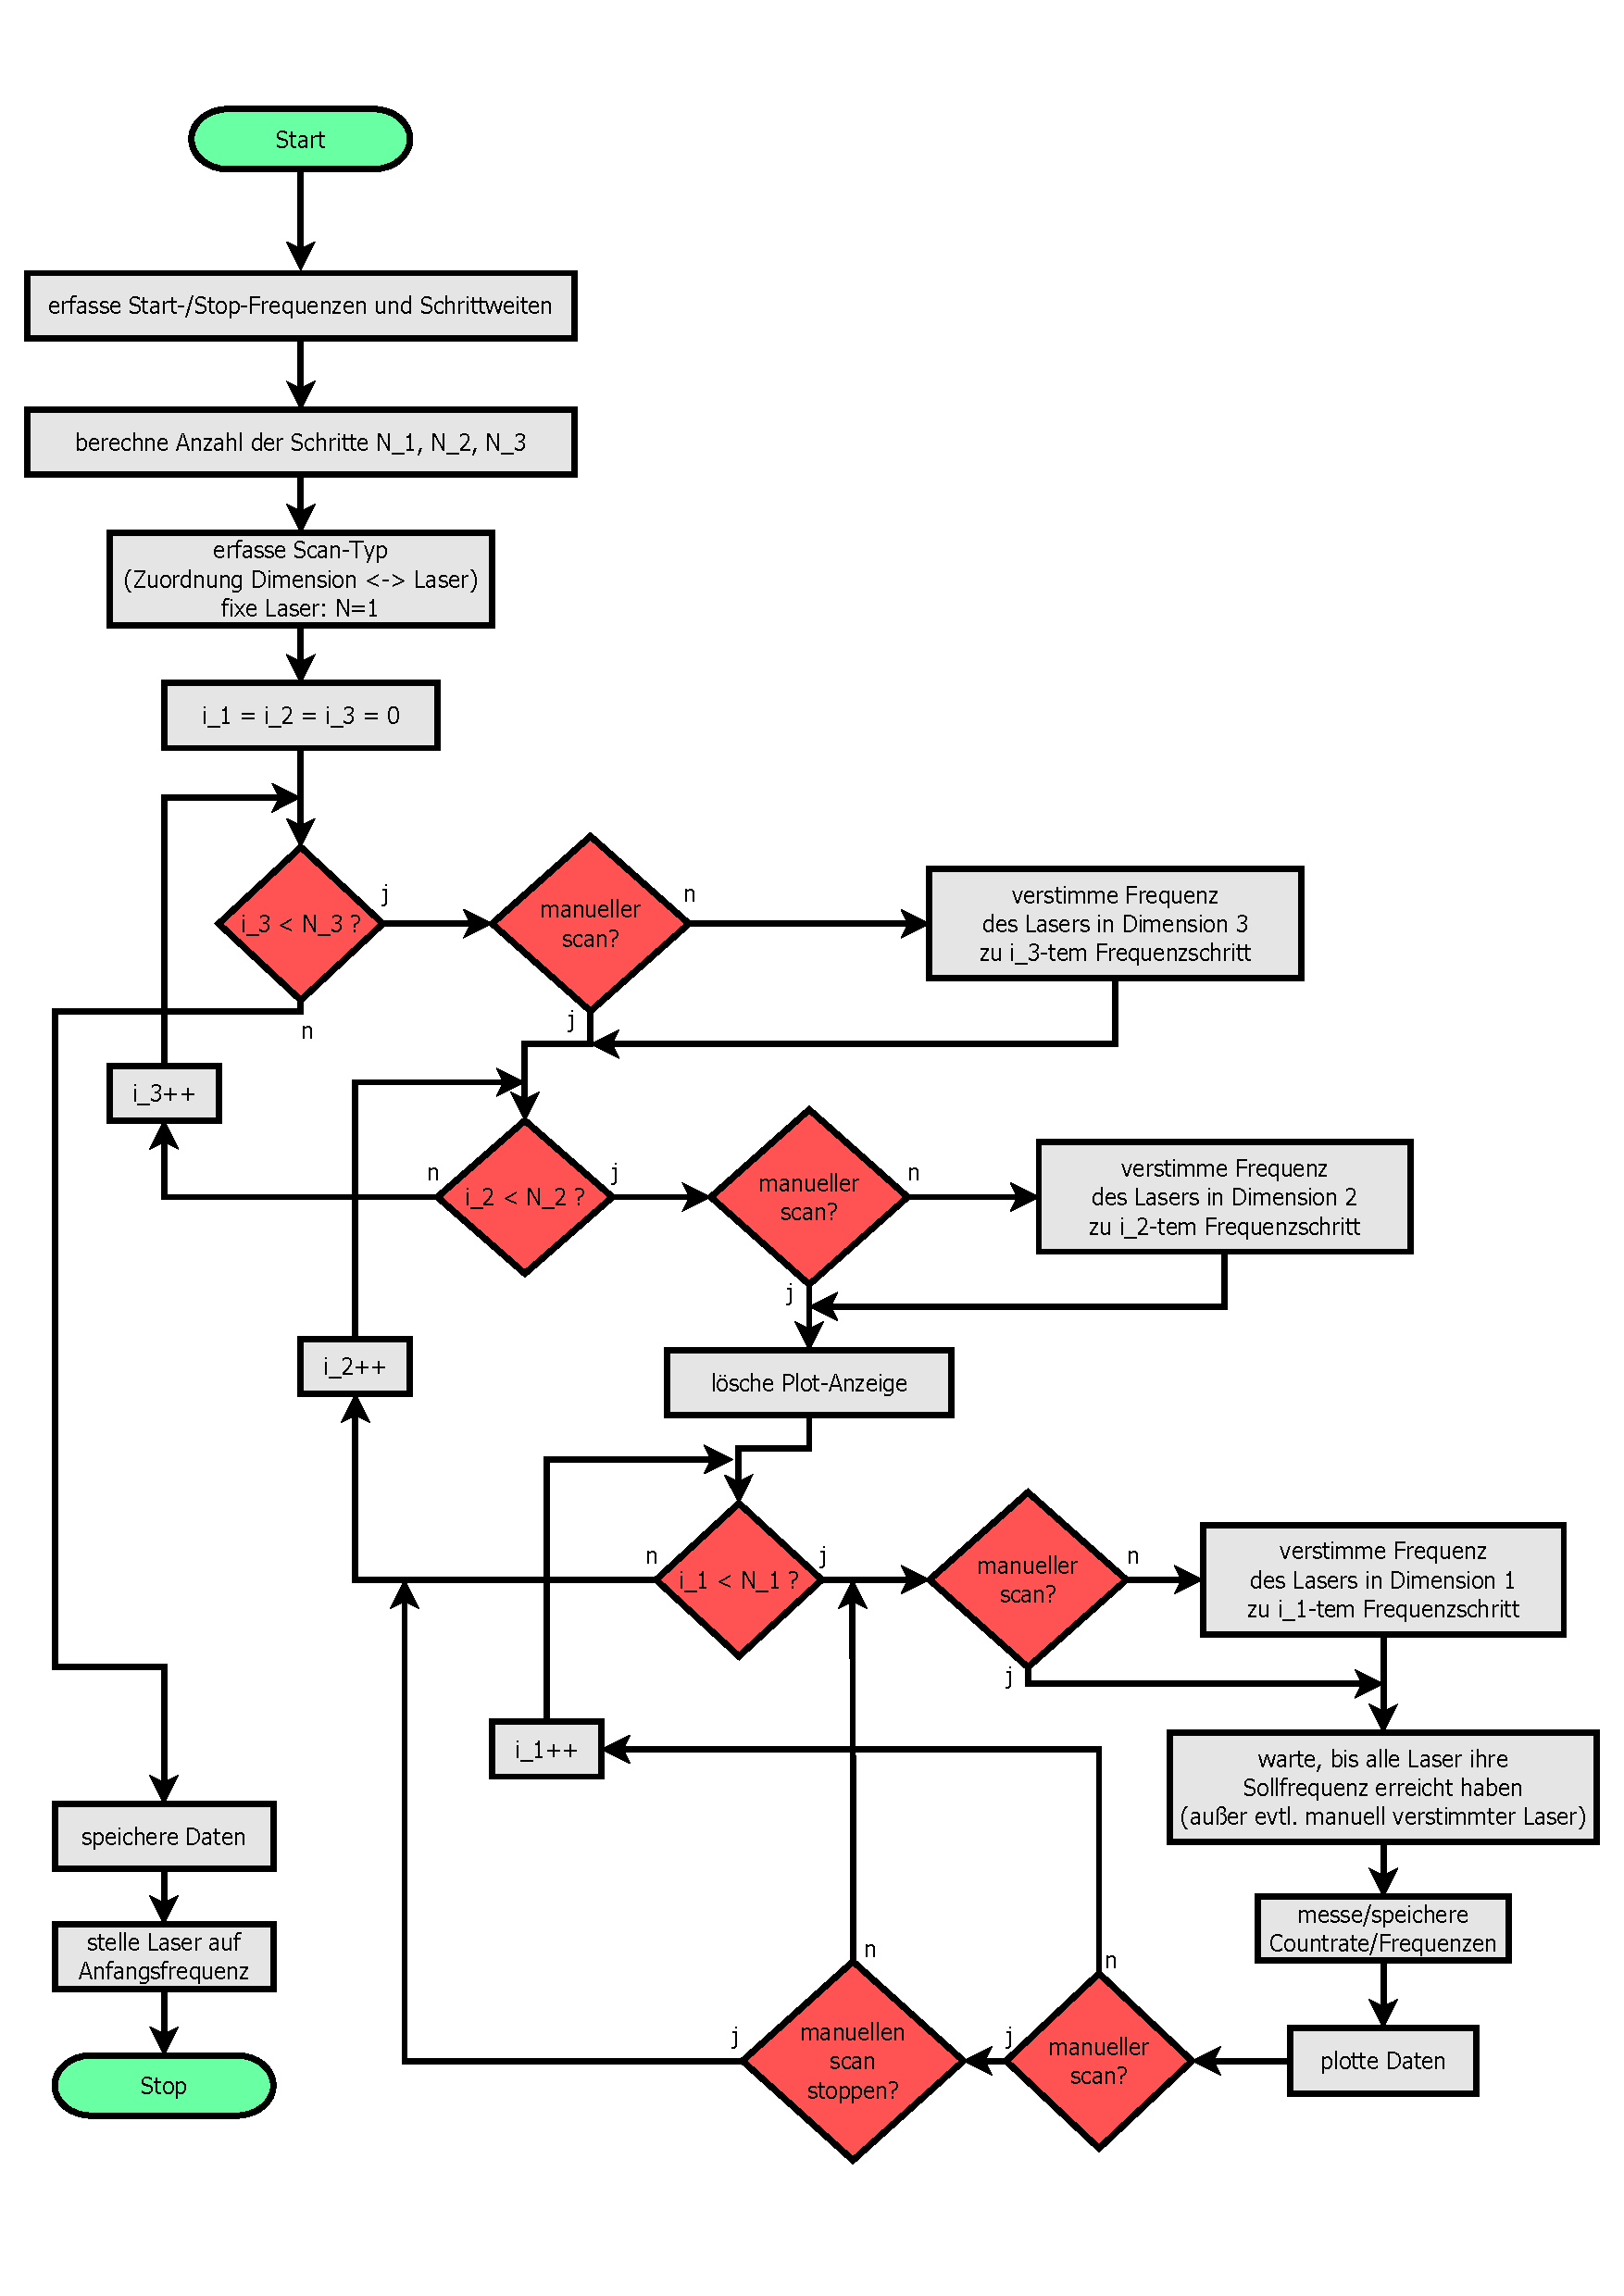
\includegraphics[width=\textwidth-0.5cm]{gfx/spektroskopie_ablaufdiagramm}
	    }}
	\caption[Spektroskopie -
	Software-Ablaufdiagramm]{Ablaufdiagramm der Spektroskopie-Routine. (j=ja,
	n=nein)}
	\label{fig:spektroskopie_ablaufdiagramm}
\end{figure}
Zunächst werden Start- und Stop-Frequenzen und die Schrittweite der Laser
ermittelt, woraus dann die einzelnen Anzahlen der Schritte berechnet werden.
Weiterhin werden die Laser ihrer Dimension zugeordnet, wobei für fixierte
Laser die Schrittanzahl $N=1$ gilt. Die Schleifen hierfür werden
praktisch nur einmal durchlaufen, wodurch fixe Laser ihre aktuellen
Frequenzpositionen behalten.
Die drei Dimensionen werden über drei ineinander geschachtelte Schleifen abgearbeitet. Sofern der Scan nicht
manuell verläuft, wird am Anfang jeder Schleife der Laser der entsprechenden
Dimension auf die Sollfrequenz des nächsten Schrittes verstimmt. Jedes mal, bevor in die Schleife
der ersten Dimension eingetreten wird, muss der Plot auf der Benutzeroberfläche
gelöscht werden, da hier immer nur eine Dimension angezeigt werden kann. Bevor
die Countrate aufgenommen wird, muss abgewartet werden, bis alle Laser (außer
der evtl. manuell verstimmte Laser) auf der Sollfrequenz sind.
Anschließend werden die Daten aufgenommen. Wurden alle nötigen Iterationen
durchlaufen oder wird der manuelle Scan gestoppt, werden alle Daten in eine
vorher festgelegte Datei geschrieben und alle Laser auf ihre
jeweilige Ausgangsfrequenz zurückgefahren.

\section{Sonstiges}\label{sec:sonstiges}
Um das Verwalten der \textit{iScans} über den PC zu erweitern, wurde die
Möglichkeit geschaffen, alle wichtigen \textit{iScan}-Parameter über die
Benutzeroberfläche des \textit{Labview}-Programms zu editieren. Dazu gehören
die Scan-Parameter und die Parameter, die zur Modulation der
Laser-Parameter wichtig sind (siehe Abschn. \ref{subsec:iscan_control_unit}).
Weiterhin können die Streckfaktoren und Offsets der normierten Signale des
\textit{iScan heads} editiert werden. Das kann entweder manuell
oder automatisch über die Routine \textit{Circle Alignment} durchgeführt
werden. Diese Routine wurde von \textit{TEM Messtechnik übernommen} und leicht
modifiziert, damit sie in das Hauptprogramm eingebettet werden konnte. Dabei
wird der Laser mehrfach um einen \textit{iScan}-FSR in der Frequenz verstimmt
und das Quadratursignal analysiert. Dadurch werden die nötigen Faktoren
berechnet, damit eine Kreissymmetrie entsteht.

%TODO: !!Ablaufdiagramme: Text größer